%# -*- coding: utf-8-unix -*-
\chapter{主观评价与眼动实验数据的处理}
\label{chap:dataprocess}
通过第\ref{chap:databaseconstruction}章的实验,我们得到了两部分数据,一是主观评分数据,二是眼动数据。下面我们分别对这两种数据集进行预处理。

\section{主观评分的处理}
\label{sec:subjectscore}
立体图像的主观评分是在眼动实验\ref{sec:stereoscopicimageeyetrackdatacollecting}中获取的,每幅图像播放10s,获取眼动数据后,眼动仪停止记录,被试将对刚才看到的图像进行评分,整个过程相当于单刺激主观评分。评分区间为1-5分,分别表示图像质量差、较差、一般、良好、优秀等五个等级。本节将首先对数据进行异常值剔除,然后通过保留的数据求对应于各幅图像的MOS值。
\subsection{主观评分异常值检测与剔除}
\label{sec:dropsinglesubjecterrorvalue}
我们的实验被试共记24人,每个人都对77副图像进行了主观评分,为了保证评分的可信度,我们需要做评分的异常值检测。
这里采用ITU-R BT.500-11\parencite{recommendation2002500}标准中针对“单刺激连续测试方法”的异常值检测算法。

第一,确定针对一幅立体图像的评分是否属于正态分布,即对一副图像的评分做${\beta _2}$检验,也称为求Kurtosis系数\parencite{goldmann2010comprehensive}。Kurtosis系数在数学上可以定义为随机变量四阶中心矩和方差平方的比值:
\begin{equation}
kurtosis = \frac{{\sum\nolimits_{i = 1}^N {{{({Y_i} - \overline Y )}^4}} }}{{(N - 1){s^4}}}
\end{equation}
\begin{figure}[htbp]
  \centering
  \begin{minipage}[b]{0.73\textwidth}
    \captionstyle{\centering}
    \centering
    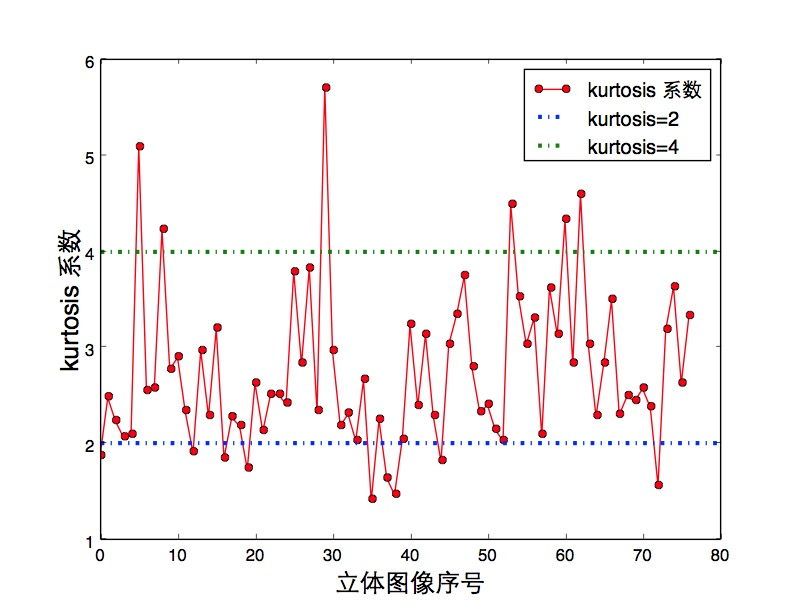
\includegraphics[width=\textwidth]{chap4/kurtosis}
    \bicaption[fig:kurtosis:a]{77幅图像对应的Kurtosis 系数以及正态分布的临界值2,4}{77幅图像对应的Kurtosis 系数以及正态分布的临界值2,4}{Fig}{Kurtosis coeficients of 77 stereoscopic image and the critical values 2,4 for normal distribution.}
  \end{minipage} %  
  \hfill
  \begin{minipage}[b]{0.74\textwidth}
    \captionstyle{\centering}
    \centering
    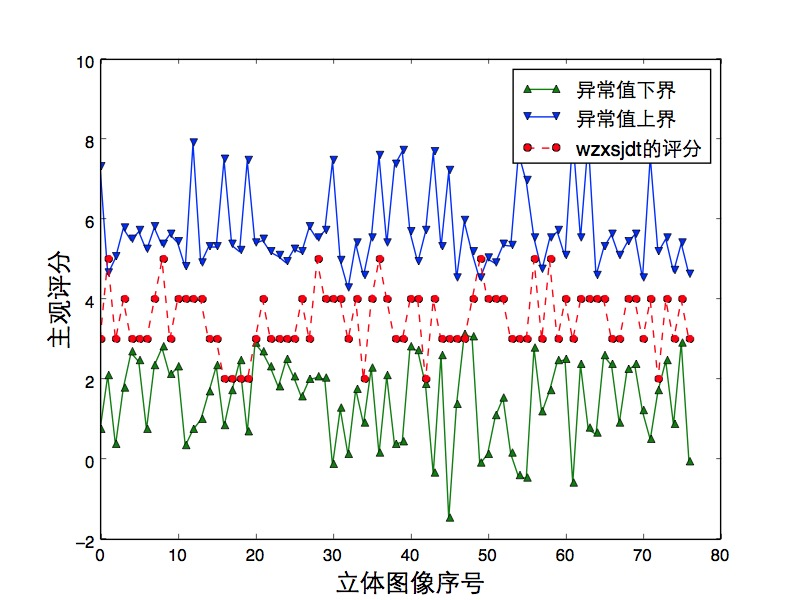
\includegraphics[width=\textwidth]{chap4/exampleofoneperson}
    \bicaption[fig:exampleofoneperson:b]{77幅图像的主观评分的异常评分上界(蓝色)和下界(绿色)以及其中一个被试的评分(红色)}{77幅图像的主观评分的异常评分上界(蓝色)和下界(绿色)以及其中一个被试的评分(红色)}{Fig}{The sup(blue) and inf(green) scores for 77 images and the scores(red) from a participant}
  \end{minipage}     
\end{figure}
这个值称为峰度,一般认为当峰度值为3时,数据组服从正太分布。\parencite{recommendation2002500}建议一组数据的峰度值在$[2,4]$之间时,认为该组数据服从正态分布,否则是非正态分布。
我们的主观数据包含77幅图像的评分,每幅图像对应评分的kurtosis系数如图\ref{fig:kurtosis:a}所示。

从图中可以看出,大部分图像的主观评分符合正态分布。

第二,确定合理主观评分的上界${\rm{supS}}$与下界${\rm{infS}}$,\parencite{recommendation2002500}建议的上下界根据评分分布是否服从正态分布可以定义为:
\begin{equation}
{\rm{supS_k = }}\left\{ \begin{array}{l}
{{\bar \mu }_k} + 2*{S_k}{\rm{\qquad              if\  distribution\  is\  normal}}\\
{{\bar \mu }_k} + \sqrt {20} *{S_k}{\rm{\qquad         otherwise}}
\end{array} \right.
\end{equation}
\begin{equation}
{\rm{infS_k = }}\left\{ \begin{array}{l}
{{\bar \mu }_k} - 2*{S_k}{\rm{\qquad              if\  distribution\  is\  normal}}\\
{{\bar \mu }_k} - \sqrt {20} *{S_k}{\rm{\qquad          otherwise}}
\end{array} \right.
\end{equation}
其中${{\bar \mu }_k} $,${S_k}$是所有被试对第$k$幅图像评分的均值与标准差,定义$P_i$,$Q_i$分别表示第$i$个被试的所有评分中超出相应图像评分的上界和下界的次数。即
\begin{equation}
\left\{ \begin{array}{l}
{P_i} = {P_i} + 1{\qquad if\ {u_{ik}} > {\rm{sup}}{{\rm{S}}_k}}\\
{Q_i} = {Q_i} + 1{\qquad if\ {u_{ik}} < {\rm{inf}}{{\rm{S}}_k}}
\end{array} \right.
\end{equation}
其中${u_{ik}}$表示第$i$个被试对第$k$幅图像的评分。
定义局部评分偏大的偏度$Bia{s_{\sup }} $与偏小的偏度$Bia{s_{\inf }}$,$M$表示被试看过的图像总数。
\begin{equation}
Bia{s_{\sup }} = \frac{{{P_i}}}{M} \qquad Bia{s_{\inf }} = \frac{{{Q_i}}}{M}
\end{equation}
根据\parencite{recommendation2002500}的建议,当\textbf{拒绝准则一}:
\begin{equation}
\label{eq:reject1}
Bia{s_{\sup }} > 20\%  \qquad or \qquad Bia{s_{\inf }} > 20\% 
\end{equation}
成立时,则拒绝被试$i$,图\ref{fig:exampleofoneperson:b}给出了其中一个被试的主观评分和图像有效评分的上下界之间的关系。我们实验的结果如图\ref{fig:distributiontestresultforall}所示。
\begin{figure}[!hbp]
  \centering
  \begin{minipage}[b]{0.49\textwidth}
    \captionstyle{\centering}
    \centering
    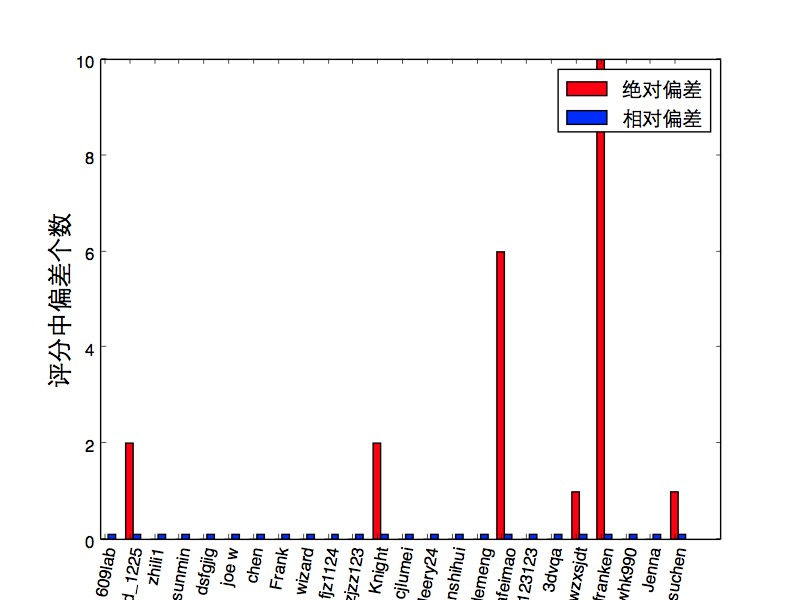
\includegraphics[width=\textwidth]{chap4/outofboundsforallperson}
    \bicaption[fig:distributiontestresultforall]{所有被试评分超出相应图像上界和下界的次数}{所有被试评分超出相应图像上界和下界的次数,这里用0.1代替0}{Fig}{Out of bounds Count for all participant, we used 0.1 instead of 0 for good performance }
  \end{minipage} %  
  \hfill
  \begin{minipage}[b]{0.49\textwidth}
    \captionstyle{\centering}
    \centering
    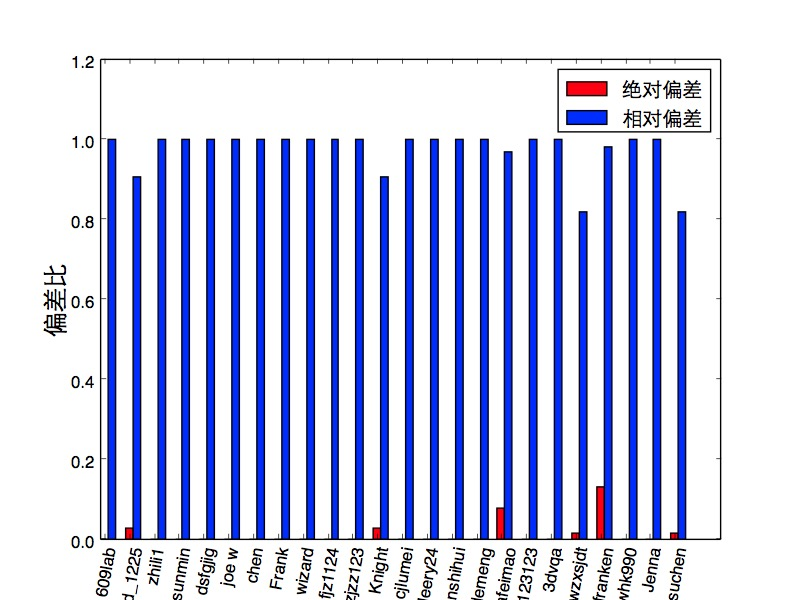
\includegraphics[width=\textwidth]{chap4/absoluteandrelativebiasforall}
    \bicaption[fig:absoluteandrelativebiasforall]{所有被试检验的绝对偏差与相对偏差}{所有被试检验的绝对偏差与相对偏差}{Fig}{The absolute bias and relative bias for all subjects}
  \end{minipage}     
\end{figure}

从图中可以看出,所有被试超出上界次数最多的是“MrFrank”,共计10次,即超出上界偏差最大$Bia{s_{\sup }}=13\%$,没有被试的评分超出下界。根据拒绝准则\ref{eq:reject1},没有用户可以被拒绝。

现在再讨论整体偏差的情况。根据\parencite{recommendation2002500}的建议,定义绝对偏差系数$Bia{s_{abs }}$与相对偏差系数$Bia{s_{relative }}$为:
\begin{equation}
\label{eq:absrelativebias}
\left\{ \begin{array}{l}
Bia{s_{abs}} = \frac{{{P_i} + {Q_i}}}{M}\\
Bia{s_{relative}} = \frac{{\left| {{P_i} - {Q_i}} \right|}}{{{P_i} + {Q_i}}}
\end{array} \right.
\end{equation}
根据\parencite{recommendation2002500}的建议,当\textbf{拒绝准则二}:
\begin{equation}
\label{eq:reject2}
\left\{ \begin{array}{l}
Bia{s_{abs}} > 10\% \\
Bia{s_{relative}} < 30\% 
\end{array} \right.
\end{equation}
成立时,拒绝当前被试$i$。图\ref{fig:absoluteandrelativebiasforall}显示没有被试的相对误差低于30\%,所以,通过上述讨论,没有用户可以被拒绝。
\subsection{图像MOS值估计}
\label{sec:mosevaluation}
通过\ref{sec:dropsinglesubjecterrorvalue}的讨论,我们得到了可以计算MOS值的有效评分。图\ref{fig:mosandconfidence}给出了每幅图像对应的MOS值及其95\%的置信区间。
\begin{figure}[ht]
  \centering
  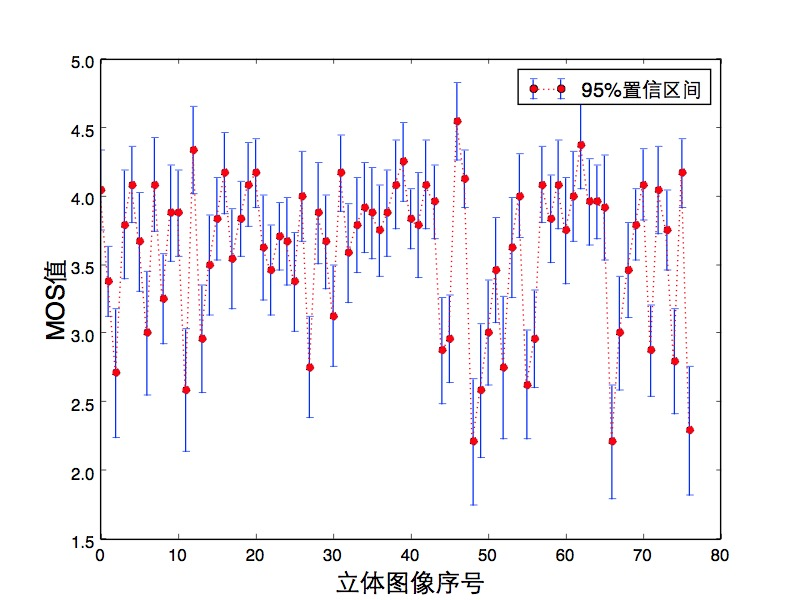
\includegraphics[width=0.6\textwidth]{chap4/mosandconfidence}
  \bicaption[fig:mosandconfidence]{77幅图对应的MOS值及其95\%的置信区间}{77幅图对应的MOS值及其95\%的置信区间}{Fig}{The MOS and 95\% confident interval for 77 images}
\end{figure}

在\ref{sec:imagedatabase}中创建图像库时本文采用了“移轴法”对选取的11幅图像进行了7种视差调整来获取不同质量的图像。现在将MOS值以相同的移轴值为基准分为7组,然后计算每个被试者对每组图像的MOS值。图\ref{fig:differentdisparity}给出了分组后的评分结果。从图中可以看出:
\begin{figure}[!ht]
  \centering
  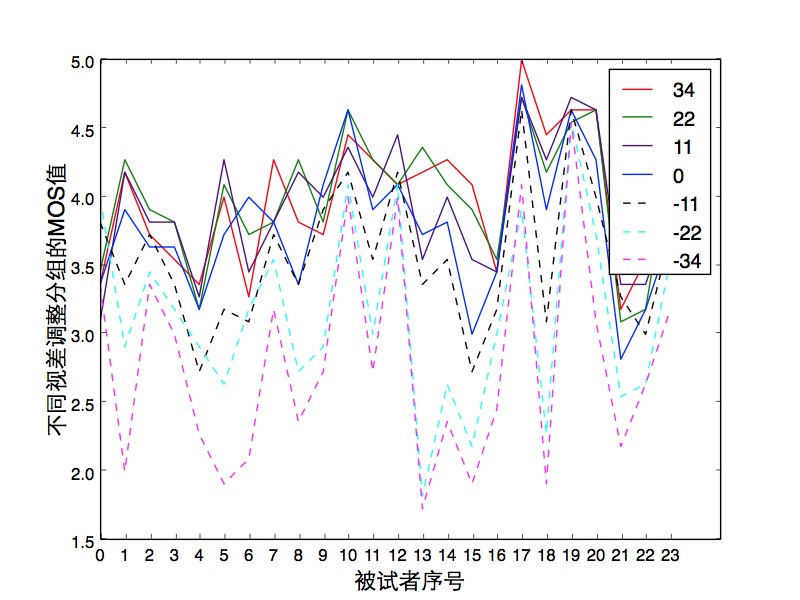
\includegraphics[width=0.6\textwidth]{chap4/differentdisparity}
  \bicaption[fig:differentdisparity]{77幅图按相同的视差调整值分组后24个被试者的MOS值}{77幅图按相同的视差调整值分组后24个被试者的MOS值}{Fig}{The MOS of different shift disparity value for 24 participants from 77 images}
\end{figure}

第一,图像的主观评分经移轴后确实产生了变化,因此,利用移轴进行视差调整确实可以创建出不同质量的图像。本文的图像库创建方法是合理的。

第二,图像从预设的最舒适的位置开始视差调整,可以看出,视差调整值为正(11,22,34)时,图像质量较好。说明图像内容相对入屏时比较舒适。相反的,当视差调整值为负(-11,-22,-34)时,图像质量偏低。这说明人眼比较习惯观看入屏效果的图像。

第三,图像调整值为正时,图像质量相差不大,这说明人眼在图像相对入屏时容错性更强。而相反的,当调整值为负时,图像质量差异比较明显。图像质量会随着视差调整值的增大而变差。如图中视差调整值为-11和-34的图像质量差别较大。这说明视差调整值为负时人眼对图像质量特别敏感,这与人类在长期的进化过程中眼睛大都看的是相对入屏的场景有关。

本节我们对单刺激主观评分进行处理,主要是对主观评分数据利用ITU-R BT.500-11的标准方法进行了异常值检测。最后结果表明,实验中主观评分的数据不满足局部偏离或整体偏离的条件,均属于可接受的评分。最后,我们获取了与77幅图像对应的MOS值及其95\%的置信区间,并对相同视差调整值下图像的MOS值分布做了分析。MOS值将在第\ref{chap:model}章基于眼动数据建立立体图像质量评价模型时使用。
\section{眼动数据处理}
\label{sec:eyetrackdataprocess}
眼动数据的处理技术我们在\ref{sec:eyetracktechnology}有过综述与介绍,在这部分数据处理中,我们将改进已经成熟的算法,使处理后的数据满足:第一,在精度与准确度方面符合实际需求,第二,适应3D场景的特点。数据的精度与眼动数据的校正过程相关,而数据的准确度则与眼动数据的滤波算法相关。

\subsection{冗余数据剔除}
\label{sec:dropoverdata}
我们的眼动数据来自两部分,第一是3D校正实验,即人眼观看屏幕上产生的随机播放的不同深度不同位置的“目标”时收集的眼动数据;第二是观看立体图像时收集的眼动数据。这两种数据都会产生冗余数据。

首先,对于3D校正实验,由于每个“目标”播放2s钟,当下一个“目标”出现时人眼需要在位置和深度上进行调节,这个过程就会产生一些实际上不在看当前“目标”的视点,如果不剔除这些数据,就会影响最终的校正结果,而校正结果则会影响该被试测量的所有数据,这种系统性的偏差是不可接受的。为了排除这个过程的影响,我们将观看当前目标产生的眼动数据的前0.5s视为冗余数据,在实际处理中将会剔除。

对于观看立体图像时收集的眼动数据,其冗余数据会在两个时刻产生:一是刚开始时,由于我们的眼动数据收集是有任务的收集,即看完图片后还要评分,因此,这个评分的过程会影响到下次观看时人脑的调整速度,所以我们将剔除每幅图像对应眼动数据的第1s的数据。第二,观看结束时会产生冗余,我们的图片播放时长为10s,因为3D图像观看时容易产生视觉疲劳,所以到观看的后期,人的注意力会下降,这时的数据的准确性会降低。因此,我们将最后1s的数据视为冗余数据,处理时剔除。
\subsection{基于视差角的眼动数据3D校正}
\label{sec:calibraiton}
在\ref{sec:eyetrackcalibration}我们提到,眼动仪会自带一个原生的2D校正算法,实验中采用的Tobii眼动仪无论是提供给我们的studio软件还是Tobii SDK开发包,都包含了这部分功能。因此,本文对眼动仪的2D校正算法不再做讨论,而是对其3D校正过程做一下详细描述。

眼动数据的3D校正过程依赖于第三章的3D校正实验,在第三章的实验中,我们采用了25点法来替代Wang的算法\parencite{wang2014online}中的Lissajous-knot path,这25个点分别分布在5个深度平面上,每个平面上5个点的位置分别为(0.1,0.1), (0.1,0.9), (0.5,0.5), (0.9,0.1), (0.9,0.9),这里我们用(0,0)表示屏幕的左上角,而(1,1)表示屏幕的右下角。其对应的视差以像素记为-30, -10, 0, 10, 30 ,相应地视差角可以表示为$ -{0.5345^\circ }, -{0.1782^\circ }, {0^\circ }, {0.1782^\circ }, {0.5346^\circ }$,每个点在屏幕上随机播放2s。眼动仪的采样频率为60Hz,即每个目标对应120个采样点。由于采样初期人眼捕捉目标需要时间,因此,针对每个目标的数据,去掉前0.5s的采样点集,防止引入较大误差。

对于3D校正算法,在我们前面的工作中\parencite{ma2015new},采用了Wang\parencite{wang2014online}的算法,该算法可以描述为:依据预设的视差值,利用拉格朗日最小均方差\parencite{lancaster1986curve}对称的对测量视差值做平移与尺度变换,这里称该算法为基于视差偏差的3D校正算法。对于每个采样点 $j$, ${D_j}$表示当前观看目标预设的视差值,而 ${D'_j}$表示眼睛实际测量到得视差值,该值可以通过双目注视点横坐标之差来估计:
\begin{equation}
\label{eq:disparitypixel}
{D'_j} = {G'_{Rx}} - {G'_{Lx}},
\end{equation}
这里$G'_{Rx}$ 表示右眼注视点在屏幕上的横坐标,而 $G'_{Lx}$ 表示左眼注视点的屏幕上的横坐标。 用一个一阶模型来最小化测量值与预设值之间的误差,假设${a_0}, {a_1}$表示一阶模型的未知项,则该模型可以表示为:
\begin{equation}
[{d_j}] = [1\;\;{d'_j}]{\left[ {{a_0}\;\;{a_1}} \right]^T}.
\end{equation}
其中${d_j},{d'_j}$分别表示测试时刻$j$的预设视差与测量视差。这样,就可以构造一个线性系统:
\begin{equation}
\textbf{D} = \textbf{D}'\textbf{a}
\end{equation}
这里$\textbf{D}$表示已知的视差值(pixel) ,$\textbf{D}'$ 是根据眼动数据计算的视差值(pixel)。由于已知条件个数超过了未知数的个数,所以该线性系统在这里是过约束的,其解为:
\begin{equation}
\textbf{a} = {({\textbf{D}'^T}\textbf{D}')^{-1}}{\textbf{D}'^T}\textbf{D}
\end{equation}
至此,视差的校正结果可以描述为:
\begin{equation}
\label{eq:3dcalibration}
{D_j} = {a_0} + {a_1}*{D'_j}.
\end{equation}
现在将校正过的视差值反馈到左右注视点,根据方程\ref{eq:3dcalibration}可以得到眼动数据测量值的偏差:
\begin{equation}
\label{eq:errorcal}
{\varepsilon_j} = {D_j} - {D'_j}
\end{equation}
将偏差均匀的补偿给左右眼,其结果为
\begin{equation}
\label{eq:servertoeye}
\left\{ \begin{array}{l}
{G_{Lx}} = {{G'}_{Lx}} - \varepsilon_j /2,\\
{G_{Rx}} = {{G'}_{Rx}} + \varepsilon_j /2.
\end{array} \right.
\end{equation}

现在来改进该算法,以适应眼动数据测试条件。先来分析我们的测试条件与Wang的测试条件的不同,两种实验条件见图\ref{fig:conditioncompare}。
\begin{figure}
  \centering
  \subfigure[我们的测试场景]{
    \label{fig:ourcondition:a} %% label for first subfigure
    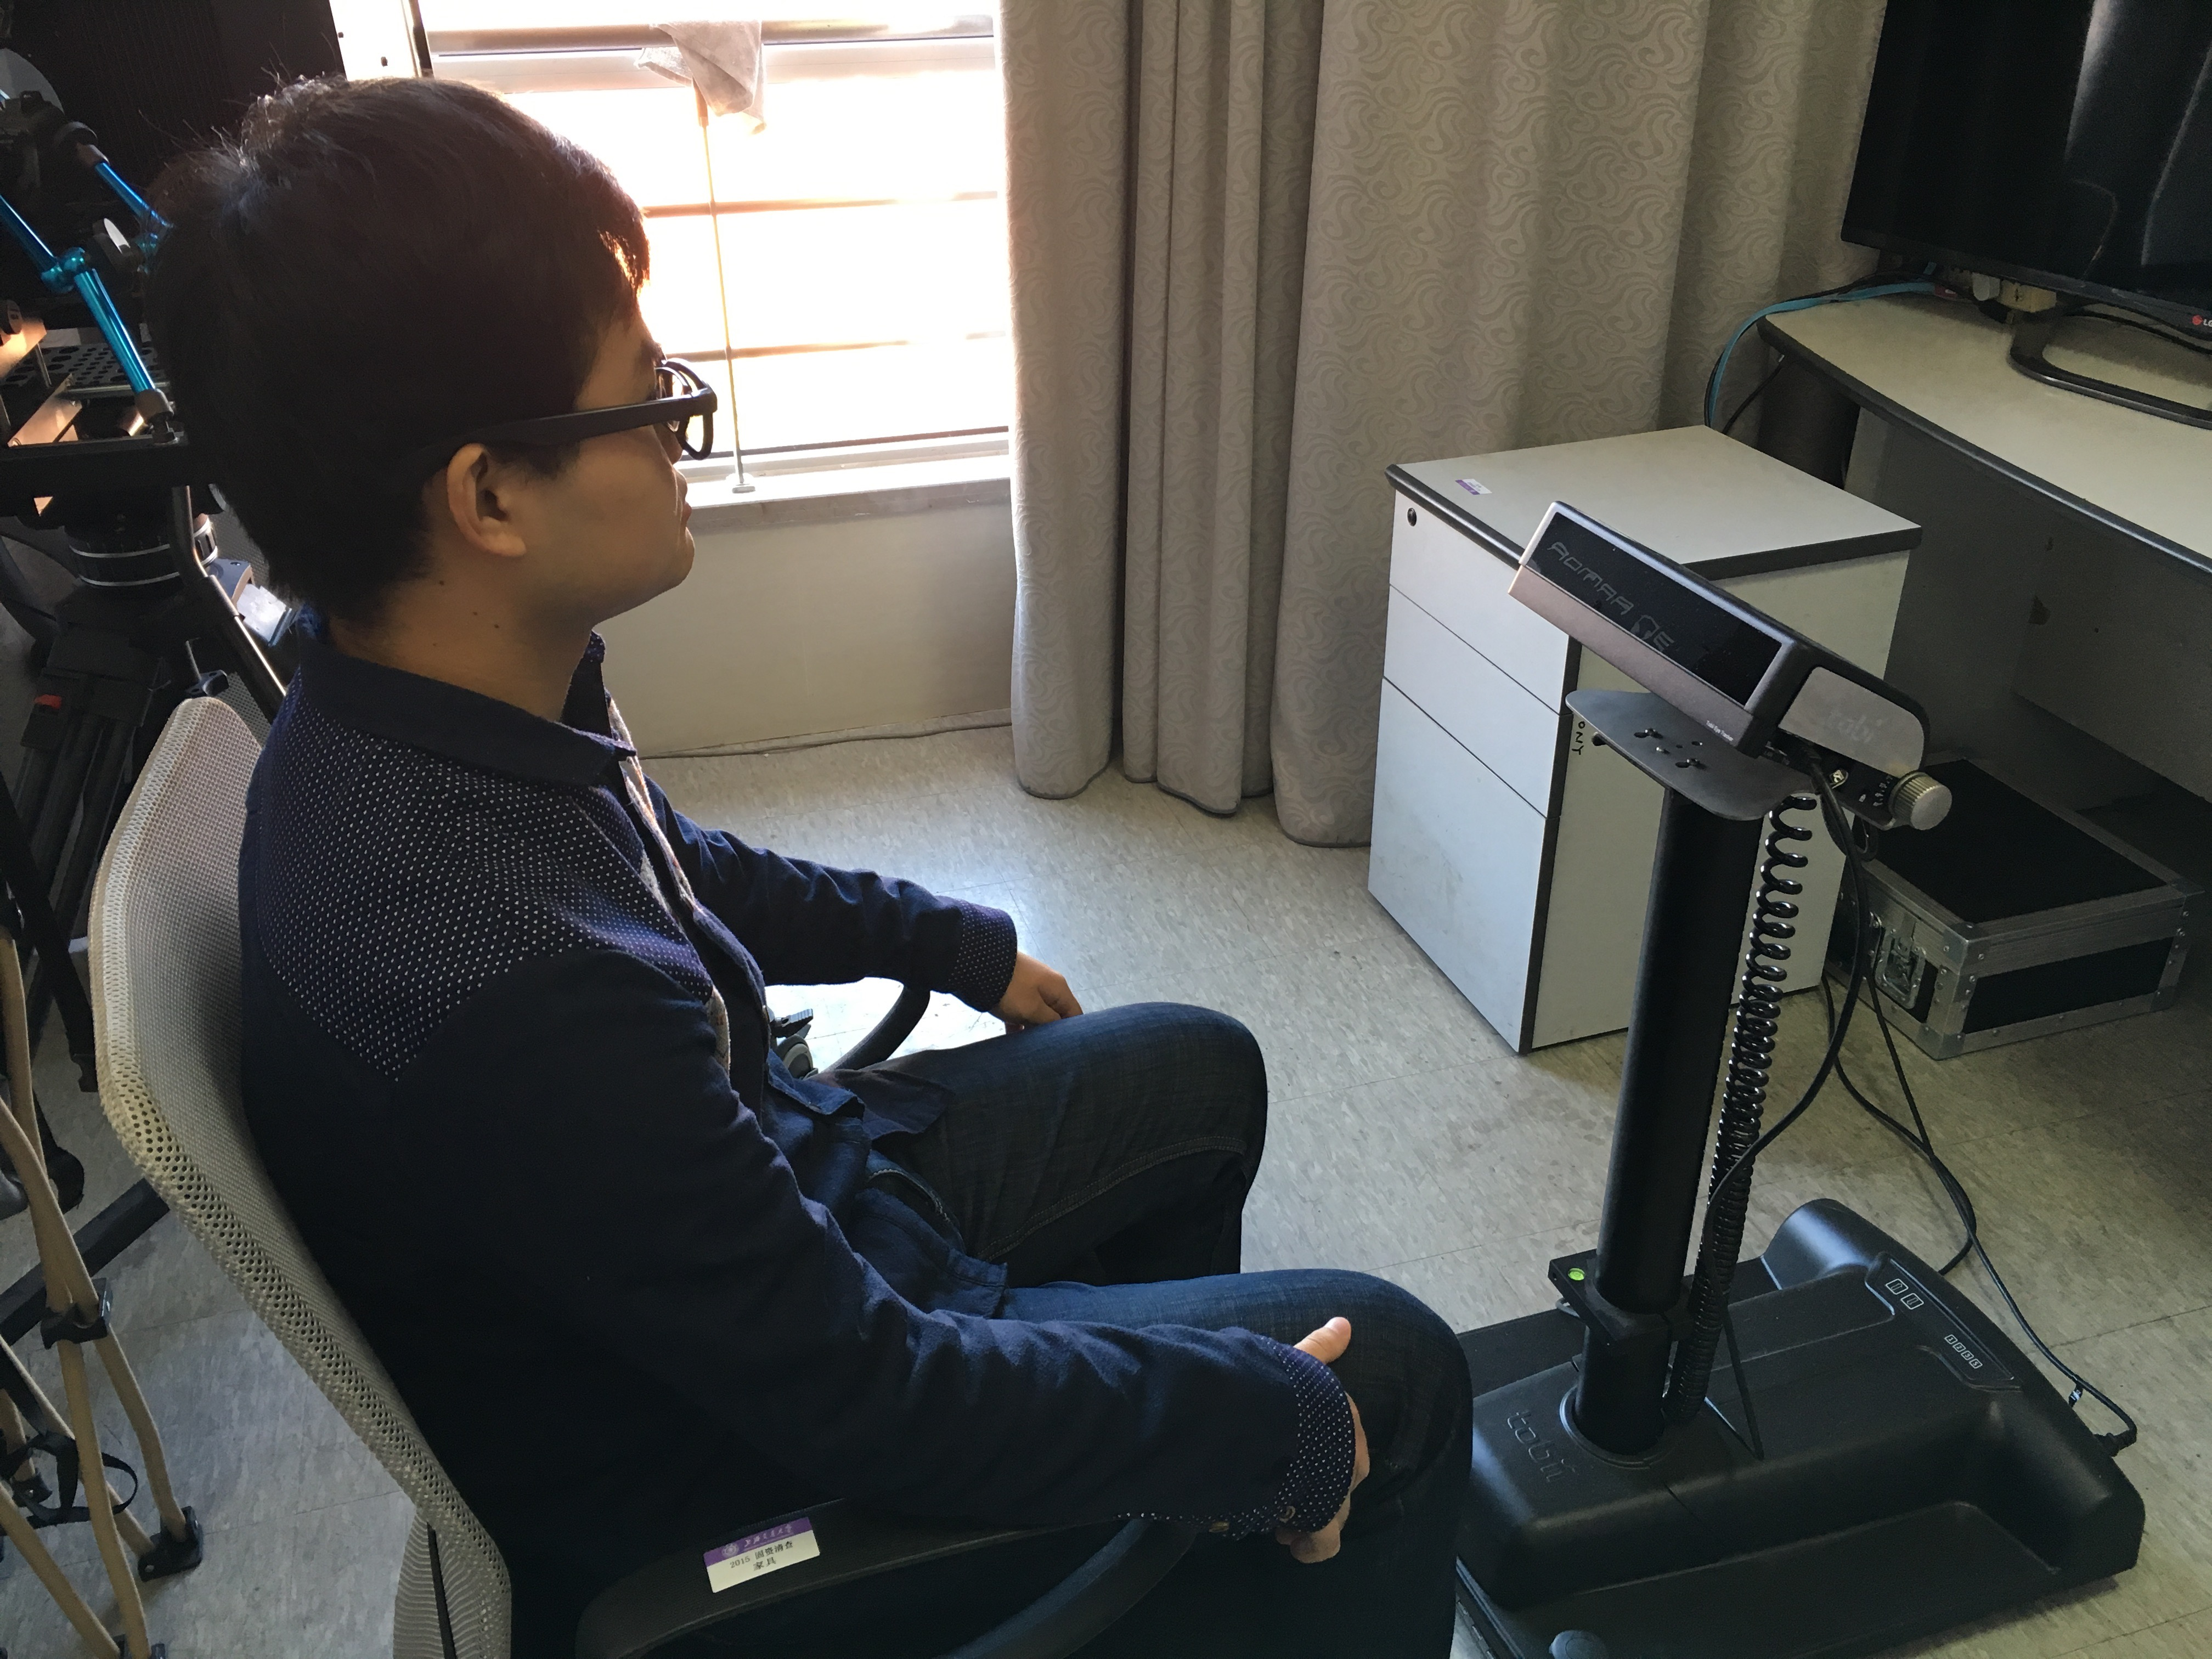
\includegraphics[width=0.3\textwidth]{chap4/ma.jpg}}
  \hspace{1in}
  \subfigure[Wang的测试场景]{
    \label{fig:wangcondition:b} %% label for second subfigure
    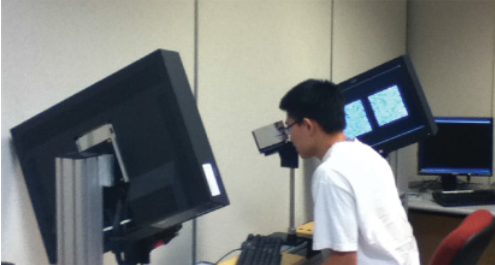
\includegraphics[width=0.4\textwidth]{chap4/wang.png}}
  \bicaption[fig:conditioncompare]{两种数据采集场景对比}{两种数据采集场景对比}{Fig}{The difference between Wang's and our condition}
\end{figure}
\begin{figure}[t]
  \centering
  \subfigure[校正前的测量数据]{
    \label{fig:beforecalibration:a} %% label for first subfigure
    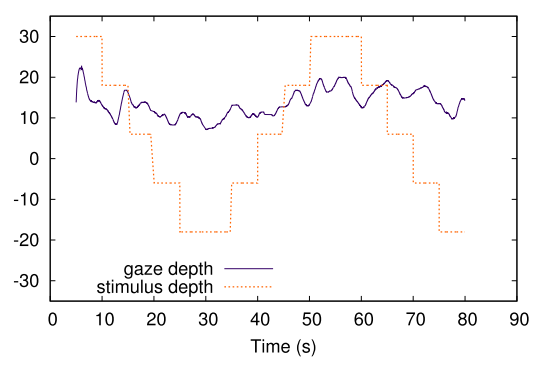
\includegraphics[width=0.45\textwidth]{chap4/beforecalibration.png}}
  \subfigure[校正后的数据]{
    \label{fig:aftercalibration:b} %% label for second subfigure
    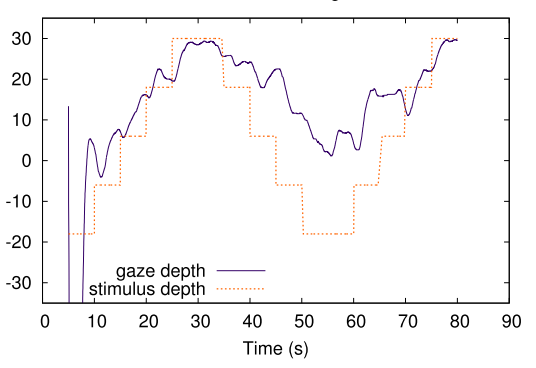
\includegraphics[width=0.45\textwidth]{chap4/aftercalibration.png}}
  \bicaption[fig:performanceofcalibration]{校正前后的效果对比图}{校正前后的效果对比图}{Fig}{The performance between before and after calibration}
\end{figure}
由图\ref{fig:conditioncompare}可见,Wang的眼动仪与头部的位置相对固定,是准侵入式设备。而我们的眼动仪则是非侵入式装备,两者的最大区别在于头部是否可动。在\ref{sec:caldisparity}中本文曾经分析了与视差角相关的量:眼睛的位置和屏幕上的注视点的位置。可见在Wang的测试条件下,由于眼睛位置相对来说比较固定,所以视差实际上由屏幕上的注视点来确定,这就是Wang的算法直接采用方程\ref{eq:disparitypixel}计算视差的原因。而我们的实验条件决定了人的头部是可动的,这就使得眼睛的位置相对不太固定,如此,直接采用方程\ref{eq:disparitypixel}计算视差的精度较低。所以,本文的算法对视差信息的估计采用视差角来表示,见方程\ref{eq:disparityofeyetrackdata}。

我们的改进方法称为基于视差角偏差的3D校正算法:
第一,利用方程\ref{eq:disparityofeyetrackdata}求得预设的视差角$\theta_j$和实际测量的视差角$\theta'_j$,仍然用一个线性系统来进行平移与尺度变换。设未知参数为$\textbf{a} = \left[ \begin{array}{l}
a\\
b
\end{array} \right]$,则此时线性系统可以表述为
\begin{equation}
\Phi  = \Phi '\textbf{a}
\end{equation}
这样我们就可以利用已知量得到该系统的解为:
\begin{equation}
\textbf{a} = {({\Phi'^T}\Phi')^{-1}}{\Phi'^T}\Phi
\end{equation}
其中$\Phi'=[\theta'_j],\Phi=[\theta_j]$.此时,视差角的校正过程如下:
\begin{equation}
\label{eq:3dcalibrationangular}
{\theta_j} = {a_0} + {a_1}*{\theta'_j}.
\end{equation}
至此,我们得到了校正后的视差角,如何将测量的偏差补偿呢?我们利用校正后的视差角计算出其在屏幕上对应的视差值(pixel)
\begin{equation}
\label{disparityfromangulartopixel}
D(pixel) = \left[ {e - 2d*\tan (\arctan (\frac{e}{{2d}}) - \frac{\theta }{2})} \right]*\frac{{{R_x}}}{W}
\end{equation}
其中$D$是像素单位的视差,$e$是人眼双目距,可以根据双目坐标求得,$d$为人眼到屏幕的距离,$\theta$是视差角。$R_x$表示屏幕的水平像素,$W$表示屏幕的宽。
此时的偏差仍然用方程\ref{eq:errorcal}来估计,最后的校正用方程\ref{eq:servertoeye}来完成,图\ref{fig:performanceofcalibration}给出了其中一个测试者校正前后的效果。
\begin{figure}[t]
  \centering
  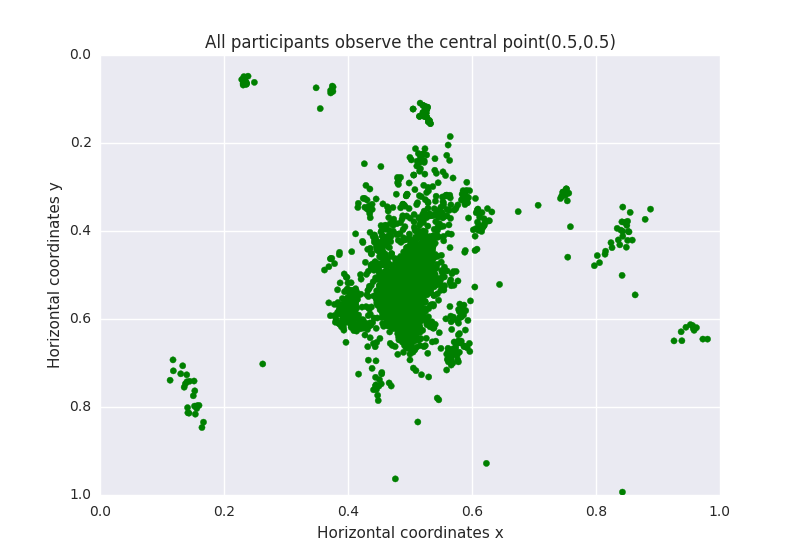
\includegraphics[width=0.5\textwidth]{chap4/rawdatadistribution}
  \bicaption[fig:rawdatadistribution]{所有实验被试观看屏幕中心点时眼睛注视点的散点图,这里我们设定屏幕左上角为(0,0),右下角为(1,1)}{所有实验被试观看屏幕中心点时眼睛注视点的散点图,这里我们设定屏幕左上角为(0,0),右下角为(1,1)}{Fig}{The scatter map of all gazepoints from participant,where(0,0)denotes upper left corner while (1,1) denotes right bottom}
\end{figure}
\subsection{基于辅眼的眼动数据滤波}
\label{sec:filter}
前面已经提到了眼动过程包含三种可能的过程,即注视过程、扫视过程以及眨眼等无法被眼动仪捕捉到得过程。眼动数据滤波的主要目的是除去噪声以及从眼动数据中分离出这些过程。众所周知,当眼睛注视一个区域时,眼睛事实上一直在颤抖,这个过程称为眼颤。眼颤的结果是当人眼注视某一点时,实际上注视了环绕该点的一片区域,而眼动仪确实会记录到这些数据,如图\ref{fig:rawdatadistribution}是所有的实验参与者观看在屏幕中心的点(0.5,0.5)的散点图。从图中可以看出,注视区域的中心与我们设定的点基本重合,但是显然,除了一些记录错误的点,其它的点都是围绕在中心注视点附近的。而这些数据就引入了噪声。因此,在眼动数据滤波这一部分,本文要解决两个问题,一个是如何确认眼动数据中的噪声以及去噪,另一个是如何从眼动数据中分离出注视过程和扫视过程。

先来分析噪声数据的类型,由于点的坐标由横纵坐标组成,我们来分析注视一个点得时候视点的横纵坐标的分布。
图\ref{fig:gazepointdistribution}给出了所有视点的横纵坐标的分布图。图\ref{fig:histmap:a}和\ref{fig:densitymap:b}清楚的表明,注视一个点时,视点的横纵坐标均符合高斯分布。即眼动数据包含的噪声表现为高斯白噪声。
因此我们在滤波时主要任务是除去数据中的高斯白噪声。
\begin{figure}[ht]
  \centering
  \subfigure[所有视点的横坐标和纵坐标分布直方图]{
    \label{fig:histmap:a} %% label for first subfigure
    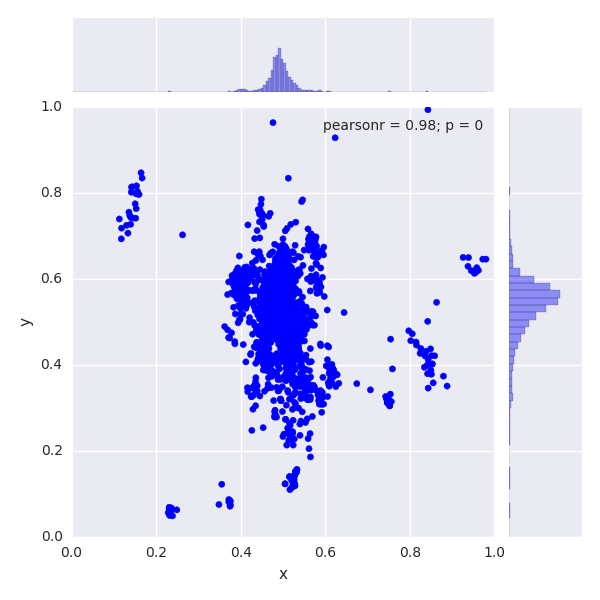
\includegraphics[width=0.47\textwidth]{chap4/eyemovehistmap}}
  \subfigure[所有视点的横坐标和纵坐标分布密度图]{
    \label{fig:densitymap:b} %% label for second subfigure
    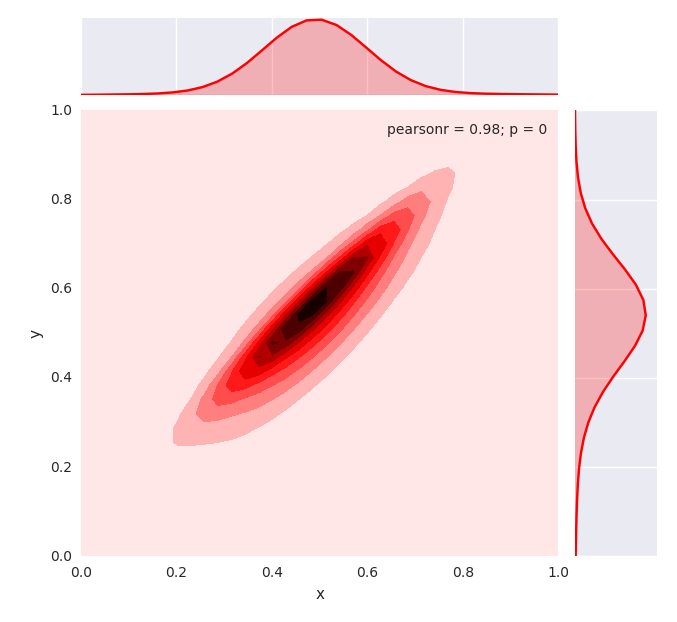
\includegraphics[width=0.47\textwidth]{chap4/eyemovedensitymap}}
  \bicaption[fig:gazepointdistribution]{所有视点的横纵坐标分布图}{所有视点的横纵坐标分布图}{Fig}{The x,y distribution of gazepoints}
\end{figure}
\parencite{duchowski2007eye}中提到,眼动过程中扫视点持续的时间大约是$30ms \sim 120ms$,注视点持续的时间是$150ms \sim 600ms$,两个扫视过程之间就是一个注视点。因此,要想分离扫视过程与注视过程,如果可以判定扫视过程,那么自然就可以判定注视过程。
扫视过程有两个特点:第一,持续时间短;第二,注视过程中会出现大的跳跃。结合这两个特征,本文仍然采用\parencite{olsson2007real}中累积距离差之和最大的方法来解决问题。我们给出这个算法的概要:

第一,根据扫视过程的持续时间,定义一个窗$L$,由于其最长持续时间是$30ms \sim 120ms$,眼动仪的采样率为60Hz,每个采样点约占16.7ms,所以一个扫视过程最少占两个采样点,最多占7个采样点,为了找出大多数的扫视点,我们取窗长为5个采样点;

第二,计算时间上相邻两个视点的距离,形成一个距离序列$D$;

第三,用长度为5的窗$L$从距离序列$D$的前五项开始,计算窗内和,让窗逐步移向$D$的尾部移动直到窗体右端到达$D$的结尾,形成窗内累积和序列$S$;

第四,当S中存在的项$s_i$满足$s_i>s_{i-1}$且$s_i>s_{i+1}$时,则此时$s_i$对应的窗内的序列就是扫视序列,相邻的区域则为注视序列。

第五,由注视序列估计注视点。由于眼动数据中的噪声为高斯白噪声,因此,取注视序列中的中值来估计该注视点,这相当于采用了中值滤波的方法来消除高斯噪声。
\begin{figure}[!htp]
  \centering
  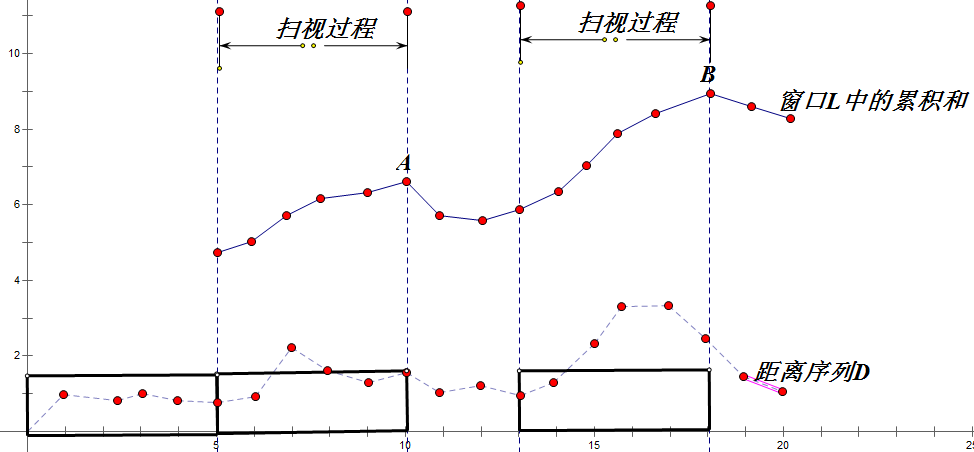
\includegraphics[width=0.6\textwidth]{chap4/windowL}
  \bicaption[fig:windowL]{基于固定窗的扫视点检验方法示意图}{基于固定窗的扫视点检验方法示意图,图中虚线是相邻两视点的欧式距离,实线为固定窗口L中的距离和。$A,B$两点满足比前后位置值都大,所以,此刻窗口对应的序列为扫视序列}{Fig}{The saccade point detecting of eyetracking data based on window L,The windows are saccade points corresponding to $A,B$}
\end{figure}
\begin{figure}[!ht]
  \centering
  \subfigure[滤波结果示意图1(主眼)]{
    \label{fig:filterresults:a} %% label for first subfigure
    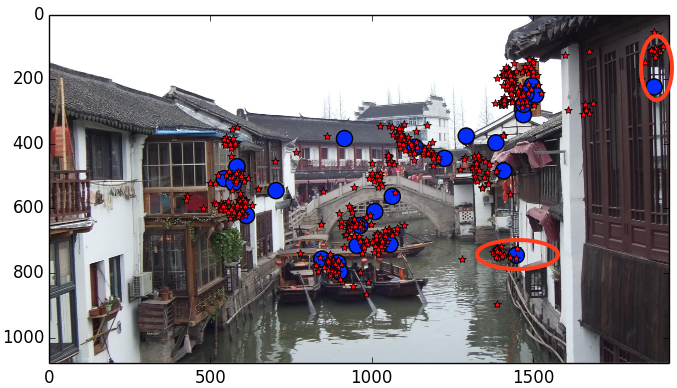
\includegraphics[width=0.45\textwidth]{chap4/filterresults2_R}}
  \subfigure[滤波结果示意图1(辅眼)]{
    \label{fig:filterresults:b} %% label for second subfigure
    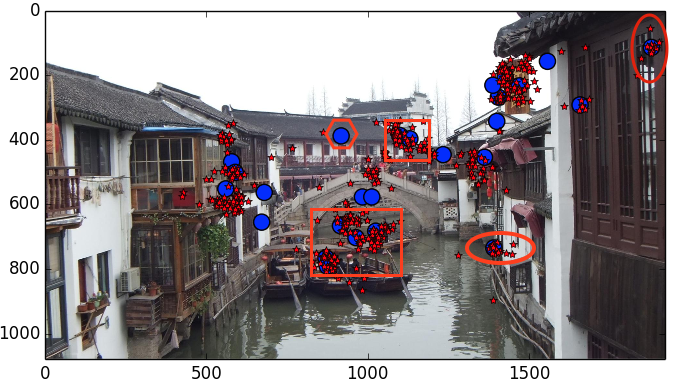
\includegraphics[width=0.45\textwidth]{chap4/filterresults2_L}}
      \subfigure[滤波结果示意图2(主眼)]{
    \label{fig:filterresults:c} %% label for first subfigure
    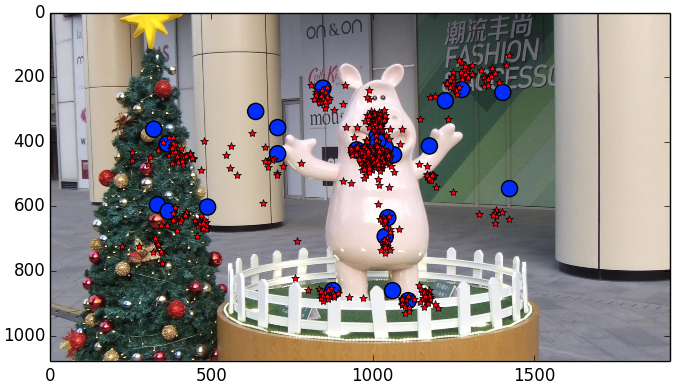
\includegraphics[width=0.45\textwidth]{chap4/filterresults3_R}}
  \subfigure[滤波结果示意图2(辅眼)]{
    \label{fig:filterresults:d} %% label for second subfigure
    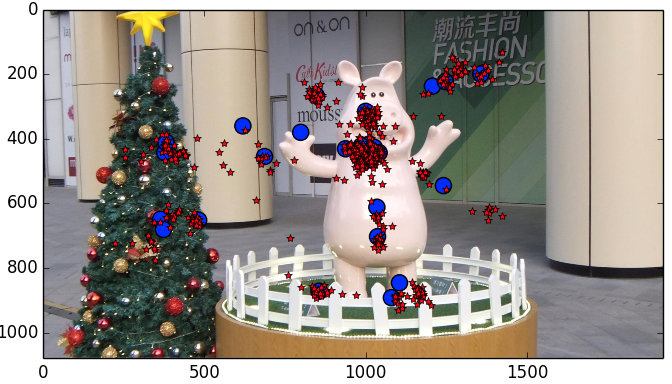
\includegraphics[width=0.45\textwidth]{chap4/filterresults3_L}}
  \subfigure[滤波结果示意图3(主眼)]{
    \label{fig:filterresults:e} %% label for first subfigure
    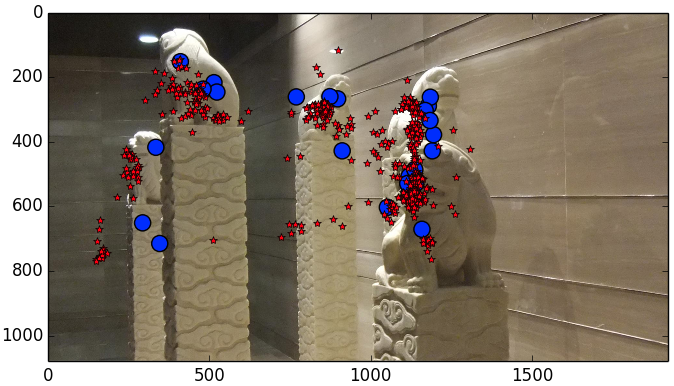
\includegraphics[width=0.45\textwidth]{chap4/filterresults4_R}}
  \subfigure[滤波结果示意图3(辅眼)]{
    \label{fig:filterresults:f} %% label for second subfigure
    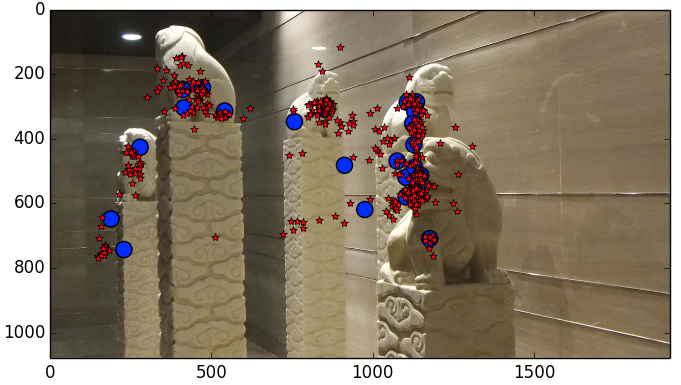
\includegraphics[width=0.45\textwidth]{chap4/filterresults4_L}}
  \bicaption[fig:filterresults]{同一幅图对应的眼动数据在不同参考眼睛下进行滤波与眼动过程分离后的结果}{同一幅图对应的眼动数据在不同参考眼睛下进行滤波与眼动过程分离后的结果,图a,c,e是以主眼为参考滤波的结果,图b,c,f是相应的以辅眼为参考滤波的结果。}{Fig}{The result of filtered and eyemovement seperate based on different eyes, a, c, e is the results based on main eye while b, c, f are based on auxiliary eye.}
\end{figure}

第六,以辅眼视点为参考进行滤波。在算法步骤二需要计算时间上相邻的两个视点间的距离,选用哪个眼睛作为参考眼睛是一个问题。一般在2D模式下,考虑的是人眼在屏幕上的注视点,所以,通常采用两眼注视点的平均位置作为参考。但是在3D模式下,双眼看到的图片不同,且双眼在立体视觉中的功能不同——主眼负责控制方向,辅眼辅助形成深度视觉。所以,考虑两个眼睛注视点的平均位置不太适用。到底选用主眼还是辅眼作为参考,我们对两种情形都进行了对比实验,图\ref{fig:filterresults}给出了同一幅在两种参考眼睛下滤波的结果。其中左边为以主眼为参考滤波的结果示意图,右边是以辅眼为参考滤波结果示意图。图中“*”表示未处理视点(Gaze point)位置,圆圈表示估计的注视点(Fixation point)位置,这里以图\ref{fig:filterresults:a}和图\ref{fig:filterresults:b}的结果为例来做分析:

首先,从图中可以看出,本文估计的注视点大部分都位于原始视点密集的地方,如图\ref{fig:filterresults:b}中矩形标注的区域。也有少部分注视点为错误的估计,如图\ref{fig:filterresults:b}中六边形标记的区域,这可能是注视时间过短的点造成的遗留,未来的算法的改进中应该考虑去除长度太短的点。另外,有些密度大的区域的注视点过于密集,这主要与观看的时间前后有关,即某一区域在$t_1$时刻被注视,过了一段时间到$t_2$时刻又被注视,此时的注视点虽然在同一个区域,但是是不同的注视点。这也是传统的聚类算法在分离眼动过程中不可用的原因。总体来看,本文的眼动过程分离算法是有效的。

其次,来分析主眼与辅眼分别为参考的滤波结果,图\ref{fig:filterresults:a}和图\ref{fig:filterresults:b}清晰的表明,以辅眼为参考眼估计的注视点精度更高,如图中椭圆标记的区域。以上结论同时可以在图\ref{fig:filterresults:c}和图\ref{fig:filterresults:d}以及图\ref{fig:filterresults:e}和图\ref{fig:filterresults:f}中看出。

最后,在第\ref{chap:model}章中进行特征提取时,发现以辅眼为参考滤波的数据提取的特征性能更优,这也从另一方面证明了采用辅眼为参考滤波的正确性。
\subsection{立体场景下眼动数据的可视化表示}
\label{sec:densitymap}
采集好的眼动数据一般以数据库或文本的形式存储,这种表示方法对于直观分析眼动结果没有任何作用。而可视化的表示方法则可以清楚地描述眼睛注视的区域,注视过程等。立体图像的眼动数据如何可视化表示呢,这是本小节要解决的问题。

一种可选的方法是直接选择传统的2D眼动数据注视密度图——灰度图与伪彩色图。图\ref{fig:2ddensitymap:b}和\ref{fig:2ddensitymapgray:c}分别是所有的被试观看实验图片\ref{fig:origimage:a}的眼动数据注视密度图,从图上可以很清楚的获取人眼注视的区域等信息。

但是,正如在\ref{eyetrackdatarepresentation}讨论的一样,3D场景下,除了2D信息之外,还包括了立体视觉最重要的信息之一——深度信息。但是上述两种方法都不能有效的表示出深度信息。因此,本节将提出一种为立体图像创建注视密度图的表示方法——3D图像注视密度图(Fixation density map)。此方法首先提出一种新的3D图像的表示方法,然后在此基础上将眼动数据依据图像分层深度也进行分层,并创建相应层的2D注视密度图,最后将各层分布在对应的深度层上形成立体表示。
\begin{figure}[!t]
  \centering
    \subfigure[伪彩色图示意图]{
    \label{fig:2ddensitymap:b} %% label for first subfigure
    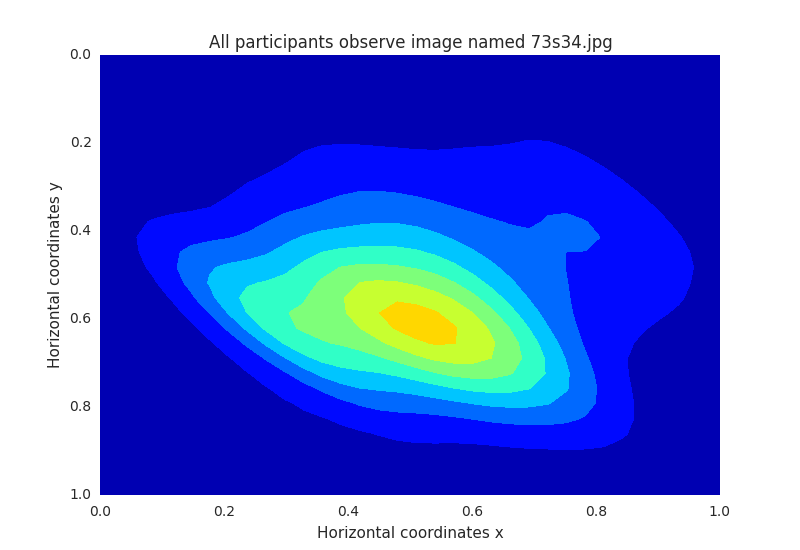
\includegraphics[width=0.4\textwidth]{chap4/2ddensitymap}}
  \subfigure[灰度图示意图]{
    \label{fig:2ddensitymapgray:c} %% label for second subfigure
    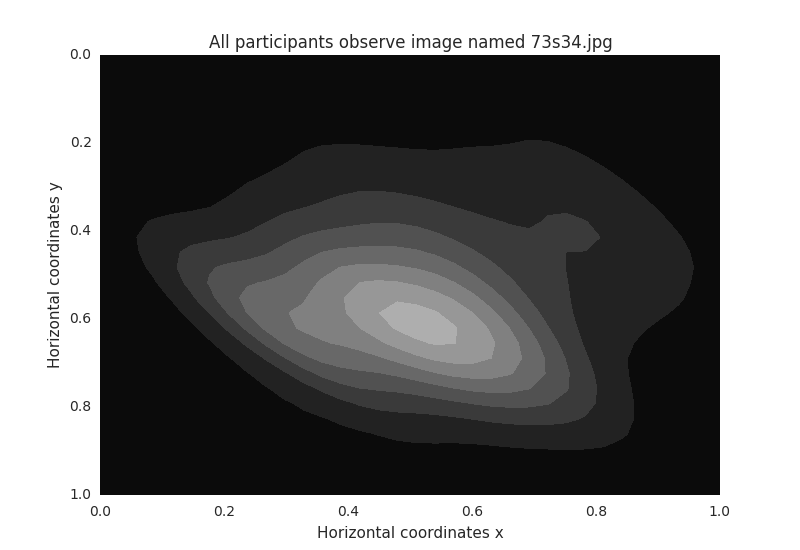
\includegraphics[width=0.4\textwidth]{chap4/2ddensitymapgray}}
    \subfigure[示意图73s34.jpg]{
    \label{fig:origimage:a} %% label for first subfigure
    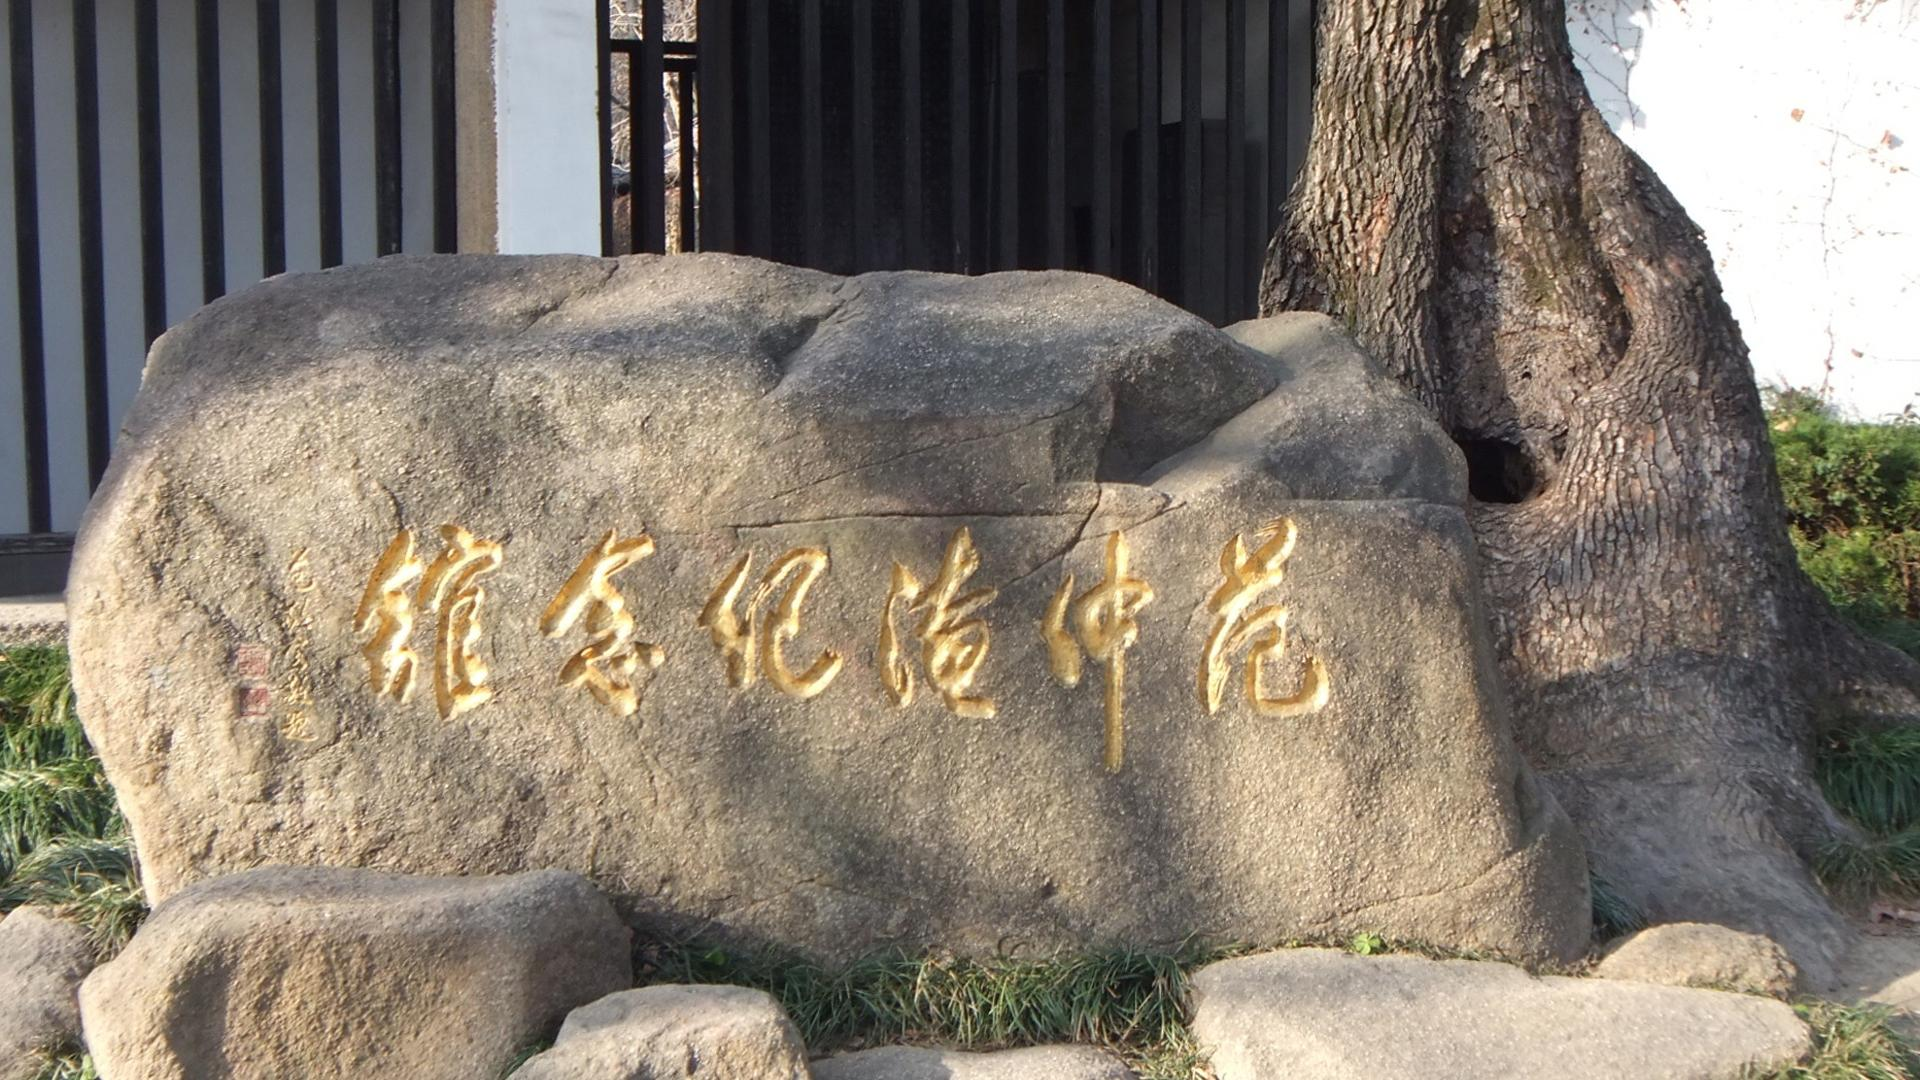
\includegraphics[width=0.5\textwidth]{chap4/73s34}}
  \bicaption[fig:densityexample]{2D眼动数据图常见的表示方法}{2D眼动数据图常见的表示方法}{Fig}{The common method to create density map for 2D image}
\end{figure}
\subsubsection{基于视差图分割的立体图像分层分割的立体表示方法}
\label{sec:stereoscopicimagerepresentation}
我们的目的是创建一种注视密度图,该图不仅可以反映用户看了什么地方,还可以反映出看的地方的深度。因此,需要一种图像的立体表示方法。而当前主流的 3D 图像的格式,如左右分离,左右合成,上下合成,交错格式,互补色格式,2D+depth等,从 本质上来说就是 2D 图像,其立体效果需要3D设备(如支持各种格式的显示器和偏振光片)的辅助才能感知到。所以,这些传统的方法无法满足当前的需求。因此,本文将在深度方向进行分割,依据视差图的信息,将图片近似的分割成若干个层次,这样,就可以近似的知道图像中各部分的深度信息。这种做法需要解决两个问题:第一,视差图的提取要较为准确。这是我们分割图像的基础,视差图提取越准确,则分割的越精确。当前提取3D图像深度的方法日趋成熟。Scharstein\parencite{scharstein2002taxonomy} 、Gangwal\parencite{gangwal2009depth}等都给出了精度很好地深度提取算法。Zhou\parencite{zhou2015depth}的工作的算法效果也很好,这里我们采用该算法。第二,图片在深度方法进行分割,最小的分割区间如何确定。与立体视觉相关的一个重要的视觉特征是人眼的立体视敏度,即人眼分辨在深度方向上相邻物体空间位置关系的能力。研究发现,在好的光线条件下,人眼的立体视敏度 可以达到 $2\sim6{\mathop{\rm arc\ sec}\nolimits} $(弧秒),而在一般情况下,人眼的立体视敏度可以为 2.3 arc min(弧分)\parencite{coutant1993population},这就为在深度方向上分割图像时确定分割步长提供了依据。

基于上述分析,这里先给出该方法的总体方案,该方案包括五个模块:
\begin{itemize}[noitemsep,topsep=0pt,parsep=0pt,partopsep=0pt]
\item 立体图像视差图提取模块,用于得到与该立体图像中参考图像相对应的视差图 $D$;
\item 立体图像深度区间设置模块,用于根据立体图像的视差特征及用于显示立体图
像的3D显示器及人眼观看的环境参数,设置该立体图像的整体深度区间; 
\item 立体图像深度平面设置模块,用于根据立体图像的视差分布特征及 3D 显示器
的环境参数,根据人眼立体视敏度设置合适的深度平面数及各深度平面间的深度区 间步长;
\item 深度层图像分割模板生成模块,用于依据所设置的深度平面数及深度区间步长,
利用视差图所反映的深度特征,分割得到各深度层对应的图像分割模板;
\item 参考图像区域分割及深度分层显示模块,用于利用所得到的各深度层对应的图
像分割模板对原图像进行分割,得到各深度平面上的图像内容,并将各深度平面上 的图像内容显示在一个立体空间中。
\end{itemize}
具体流程图如图\ref{fig:newrepresentationprocedure}所示
\begin{figure}[ht]
  \centering
  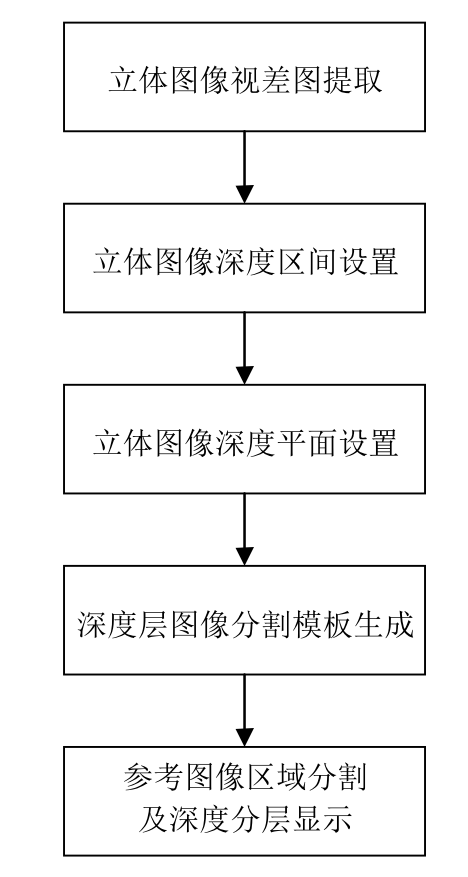
\includegraphics[width=0.3\textwidth]{chap4/newrepresentationprocedure}
  \bicaption[fig:newrepresentationprocedure]{立体图像分层表示流程图}{立体图像分层表示流程图}{Fig}{The procedure of new approach}
\end{figure}
这里我们以图\ref{fig:52L:a}为例来说明整个方法的操作过程。
\begin{figure}
  \centering
  \subfigure[示例立体图像左图]{
    \label{fig:52L:a} %% label for first subfigure
    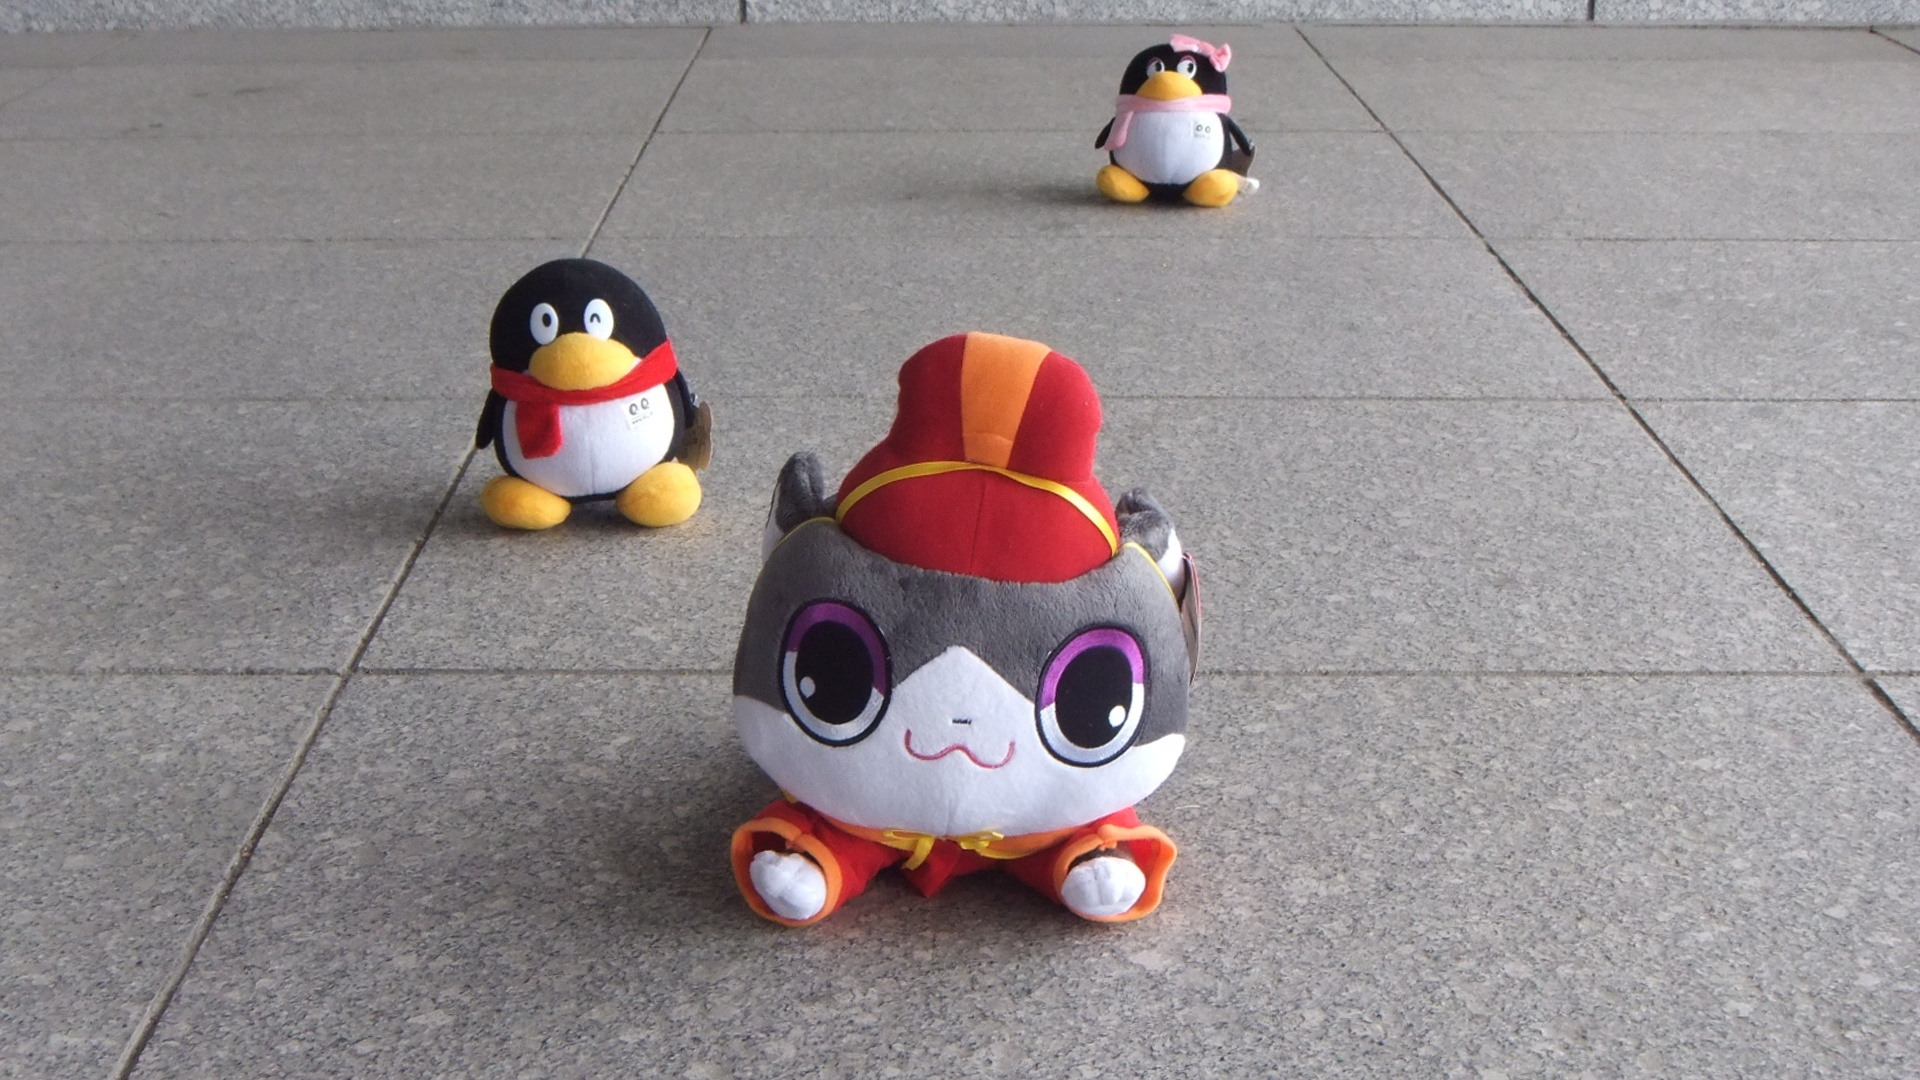
\includegraphics[width=0.4\textwidth]{chap4/52L}}
  \hspace{1in}
  \subfigure[与示例图像对应的视差图]{
    \label{fig:52_L_depthMap:b} %% label for second subfigure
    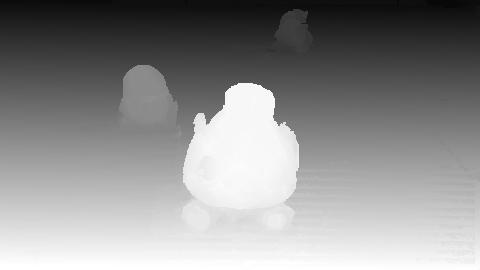
\includegraphics[width=0.4\textwidth]{chap4/52_L_depthMap}}
  \bicaption[fig:exmpleImage]{示例立体图像的左图和视差图}{示例立体图像的左图和视差图}{Fig}{The original left image and disparity map}
\end{figure}
%%%%%%%%
\\[0.2cm]
\noindent{\textbf{\emph{a.立体图像的视差提取}}}
\\[0.2cm]
\indent{本文}使用Zhou\parencite{zhou2015depth}的算法来提取视差,其效果图如图\ref{fig:52_L_depthMap:b}所示,可以看出,该算法能很好地获取立体图像的视差图。当视差信息被表征为深度图,需要按照视差图到深度图的逆映射反变换出视差图。同时,在这里得到了图像的最大视差值$D_{max}$和最小视差值$D_{min}$。
%%%%%%
\\[0.2cm]
\noindent{\textbf{\emph{b.设定深度区间}}}
\\[0.2cm]
\indent{深度}区间的设置与3D观看环境和立体图像的视差范围有关,给定3D电视及其屏幕参数,假设 $W$, $H$ 分别表示屏幕的高和宽(cm)。屏幕的分辨率可以表示为${R_x}\times{R_y}$像素。根据 ITU-R BT500-12\parencite{itu500,},人眼到屏幕的最佳距离$d$ 为3倍屏高:$d = 3*H$。另一个重要参数是人眼双目距$e$(一般认为,$e$的均值为6.5cm)。假设人眼关于屏幕中心垂线对称,就可以根据\ref{sec:stereodisparity}立体场景下视差的定义计算视差角。根据图\ref{fig:disparitydifinition},便可以获取人眼在屏幕上的汇聚角 $\alpha$:
\begin{equation}
{\alpha  = 2\arctan (\frac{e}{{2d}})}
\end{equation}
同理,可以得到双目在空间中的汇聚角$\gamma$ 或$\beta$。视差角定义为双目在屏幕上的汇聚角与在空间中的汇聚角之差。此时与视差值$D$(pixel)对应的视差角 $\theta$ 的表达式为:
\begin{equation}
\label{eq:chap4:disparitycal}
\begin{array}{l}
\theta  = 2*(\arctan (\frac{e}{{2d}}) - \arctan (\frac{{e - {D_m}}}{{2d}}))\\
{D_m} = \frac{{D*W}}{{{R_x}}}
\end{array}
\end{equation}
从\ref{eq:chap4:disparitycal}可以看出,当左右图的对应点在屏幕上的视差值  $D=0$时,视差角$\theta=0$,也就是双目汇聚在了屏幕上。
通过 \textbf{\emph{a}}部分已经得到了图像的最大最小视差值${D_{\max}}$  and ${D_{\min}}$,根据方程\ref{eq:chap4:disparitycal},就可以计算出相应的最大最小视差角$\theta _{\max }^I$和$\theta _{\min }^I$。

在这里还将考虑另一个问题,立体图像的舒适度,由于视差是影响立体图像舒适度最大的因素之一,因此,本方法将标注出舒适范围和不舒适范围。一般认为,当视差处于$( - 1^\circ , + 1^\circ )$时,图像的舒适度比较好\parencite{lambooij2009visual},超出这个范围的部分其舒适度较低。而舒适区域的部分将是我们考虑的重点。所以将分割的深度范围设定为:
\begin{equation}
(\theta _{\min }^R,\theta _{\max }^R) = (\max ( - {1^\circ },\theta _{\min }^I),\min ( + {1^\circ },\theta _{\max }^I))
\end{equation}
%%%%%%
\\[0.2cm]
\noindent{\textbf{\emph{c.决定深度分割平面}}}
\\[0.2cm]
\indent{深度}平面的个数根据图像的内容和图像在深度方向的复杂度预设为
 $M'$ ,令各相邻平面的深度区间,将深度量化区间 $Q$ 设定为人眼的立体视敏度的整数倍,即
\begin{equation}
Q = Nq = \left\lfloor{\frac{{(\theta _{\max }^R - \theta _{\min }^R)}}{{q*M'}}} \right\rfloor q
\end{equation}
这里 $\left\lfloor \cdot \right\rfloor$是向上取整算子。然后每个深度平面${P_i}$对应的视差角
 $\theta_{P_i}$ 可以表示为:
\begin{equation}
{\theta _{{P_i}}} = iQ,  i = {N_1},{N_1} + 1,...,{N_2}
\end{equation}
这里${N_1} = \left\lfloor {\theta _{\min }^R/Q} \right\rfloor,
{N_2} = \left\lfloor {\theta _{\max }^R/Q} \right\rfloor $。
此时深度平面的个数为 ${N_2} - {N_1} + 1$。除此之外,图像不总是全部在舒适范围内,因此再加两个平面,用于表示视差角处于区间 $(-\infty ,\theta_{\min }^R)$
和 $(\theta _{\max }^R, +\infty)$的部分.
最终,分割的深度平面总数为 $M = {N_2} - {N_1} + 3$。图\ref{fig:depthplaneexample}是深度平面设置的示意图。
\begin{figure}[t]
  \centering
  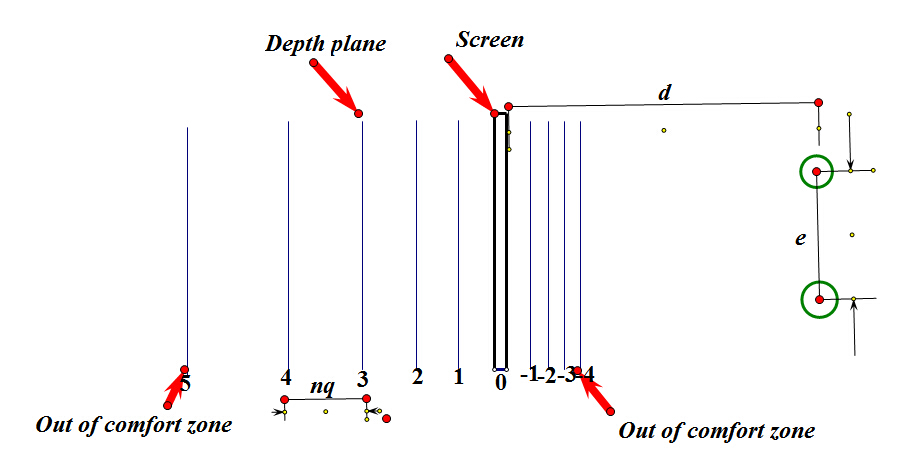
\includegraphics[width=0.7\textwidth]{chap4/depthplaneexample}
  \bicaption[fig:depthplaneexample]{深度平面设置示意图}{深度平面设置示意图}{Fig}{Example of depth levels divided in depth derection including two planes out of comfort zone}
\end{figure}
%%%%%%
\\[0.2cm]
\noindent{\textbf{\emph{d.创建立体图像分割模板}}}
\\[0.2cm]
\indent{到}目前为止,我们已经得到了立体图像的视差图和分割好的深度平面,这些平面对应的视差角都是已知的。利用这些已知的视差角来分割视差图便可以获取图像分割模板。

\uppercase\expandafter{\romannumeral1}.
考虑到深度平面 ${P_i}$的构建过程以及深度量化步长 $Q$,我们可以将深度平面${P_i}$ 对应的视差角的范围设定为:
\begin{equation}
\label{eq:depthplanedisparityrange}
{\theta _i} \in (\theta_i^- = \theta_{P_i} - \frac{Q}{2}, \theta _i^+ = \theta_{P_i} + \frac{Q}{2}].
\end{equation}
即深度平面${P_i}$ 将近似的表示视差角在${\theta _i}$范围内的图像。

\uppercase\expandafter{\romannumeral2}.
利用在\textbf{\emph{a}}部分设定的立体观看条件,可以计算出与${\theta _i}$对应的视差值的范围 ${D_i} \in (D_i^- ,D_i^+]$。
\begin{equation}
{D_{pixel}} = [e - 2d*\tan (\arctan(\frac{e}{{2d}}) - \frac{\theta}{2})]*\frac{{{R_x}}}{W}.
\end{equation}

\uppercase\expandafter{\romannumeral3}.
已知视差图$D$ 和深度平面 ${P_i}$对应的视差范围 ${D_i}$ ,我们可以获取与深度平面${P_i}$对应的图像分割模板。
\begin{equation}
{M_{{P_i}}}(x,y) = \left\{ \begin{array}{l}
1,\;\;\;\;\;\;D(x,y) \in (D_i^ - ,D_i^ + ]\\
0,\;\;\;\;\;\;otherwise
\end{array} \right.
\end{equation}
这里$D(x,y)$ 指的是视差图上 $(x,y)$处的值。由视差图\ref{fig:52_L_depthMap:b}获取的图像分割模板如图\ref{fig:segmask}所示。
\begin{figure}
  \centering
  \subfigure[]{
    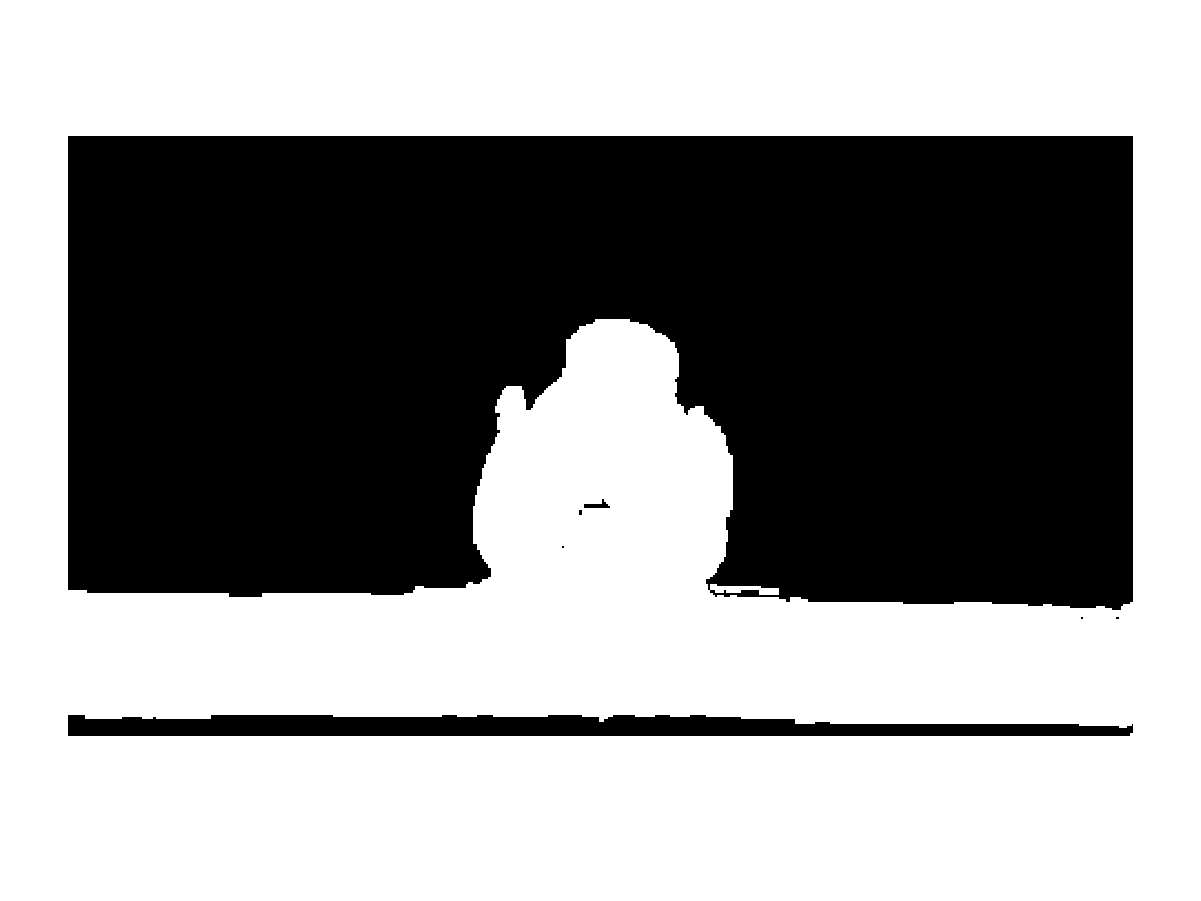
\includegraphics[width=0.16\textwidth]{chap4/depthseg1}}
  \subfigure[]{
    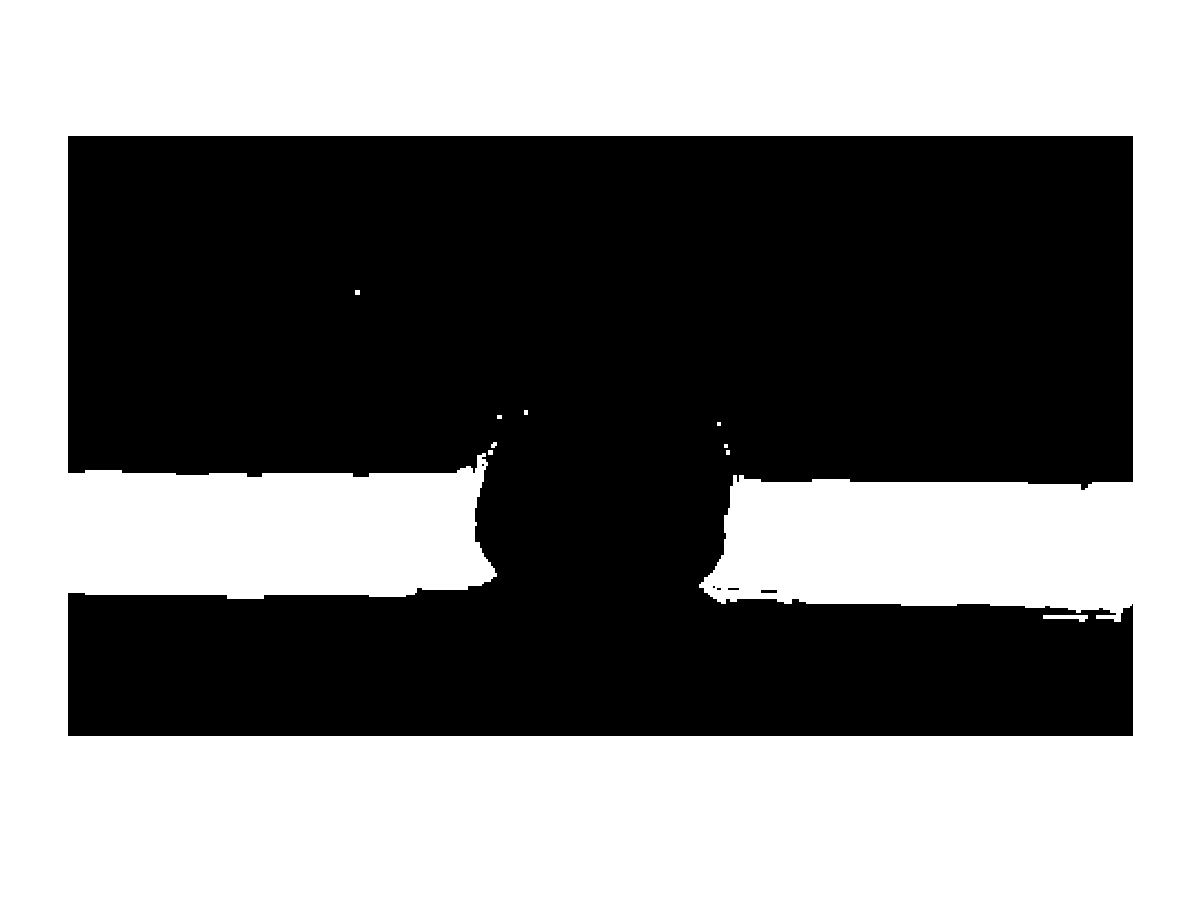
\includegraphics[width=0.16\textwidth]{chap4/depthseg2}}
  \subfigure[]{
    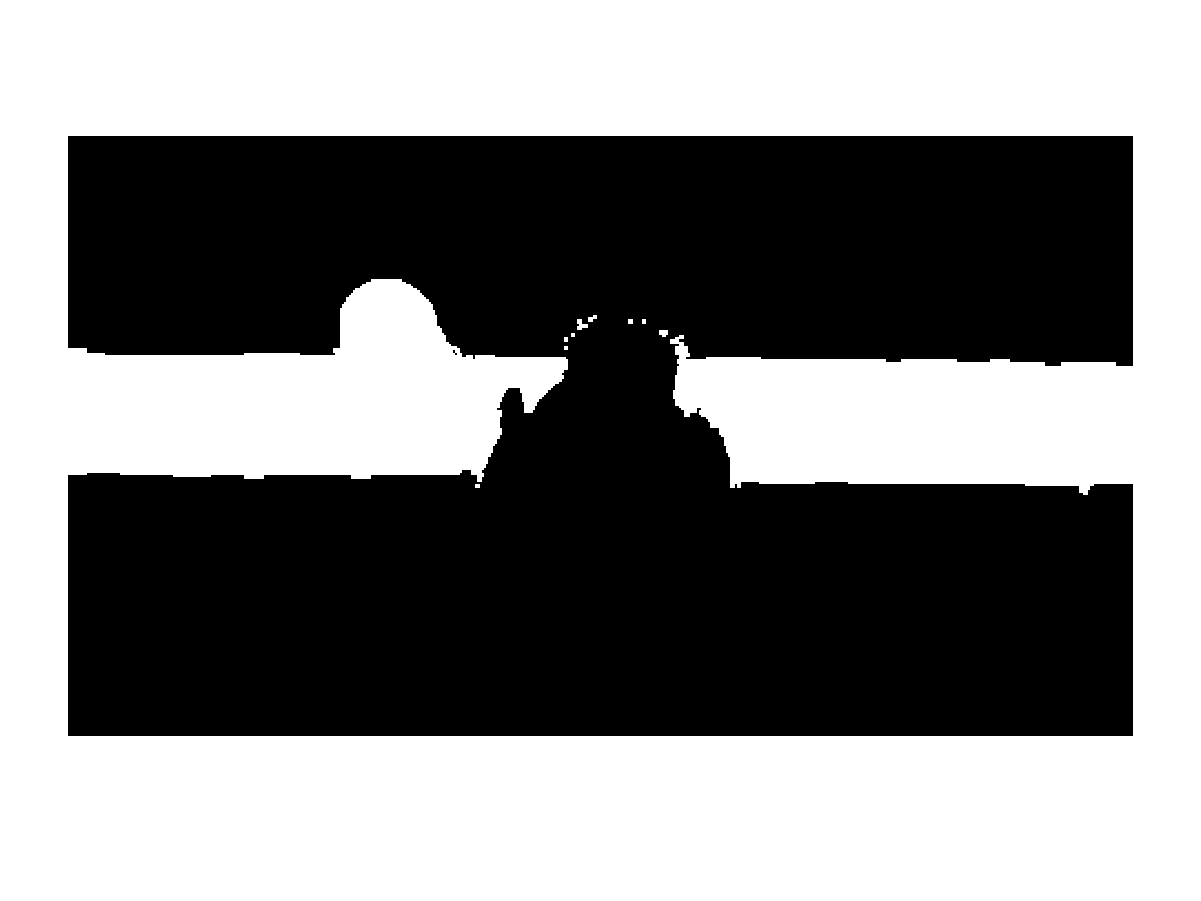
\includegraphics[width=0.16\textwidth]{chap4/depthseg3}}
  \subfigure[]{
    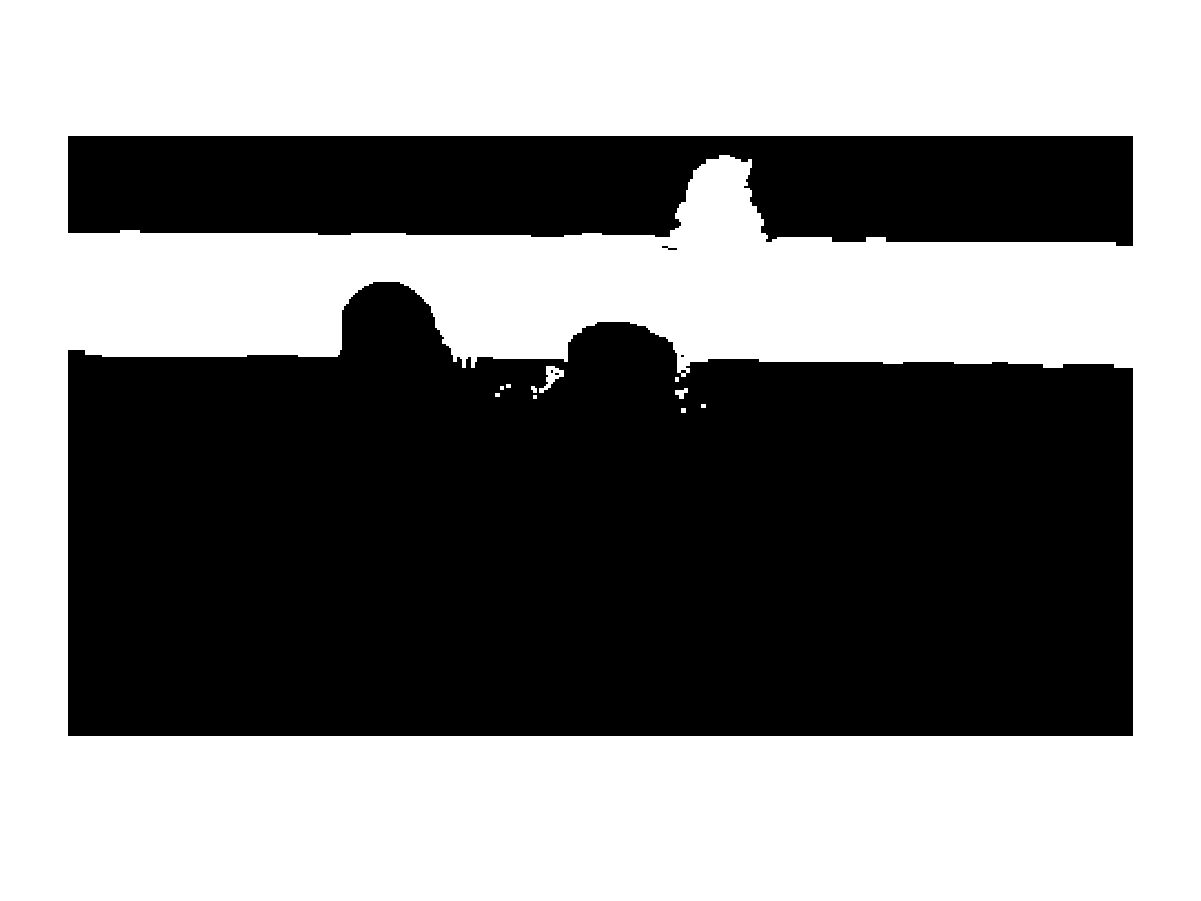
\includegraphics[width=0.16\textwidth]{chap4/depthseg4}}
  \subfigure[]{
    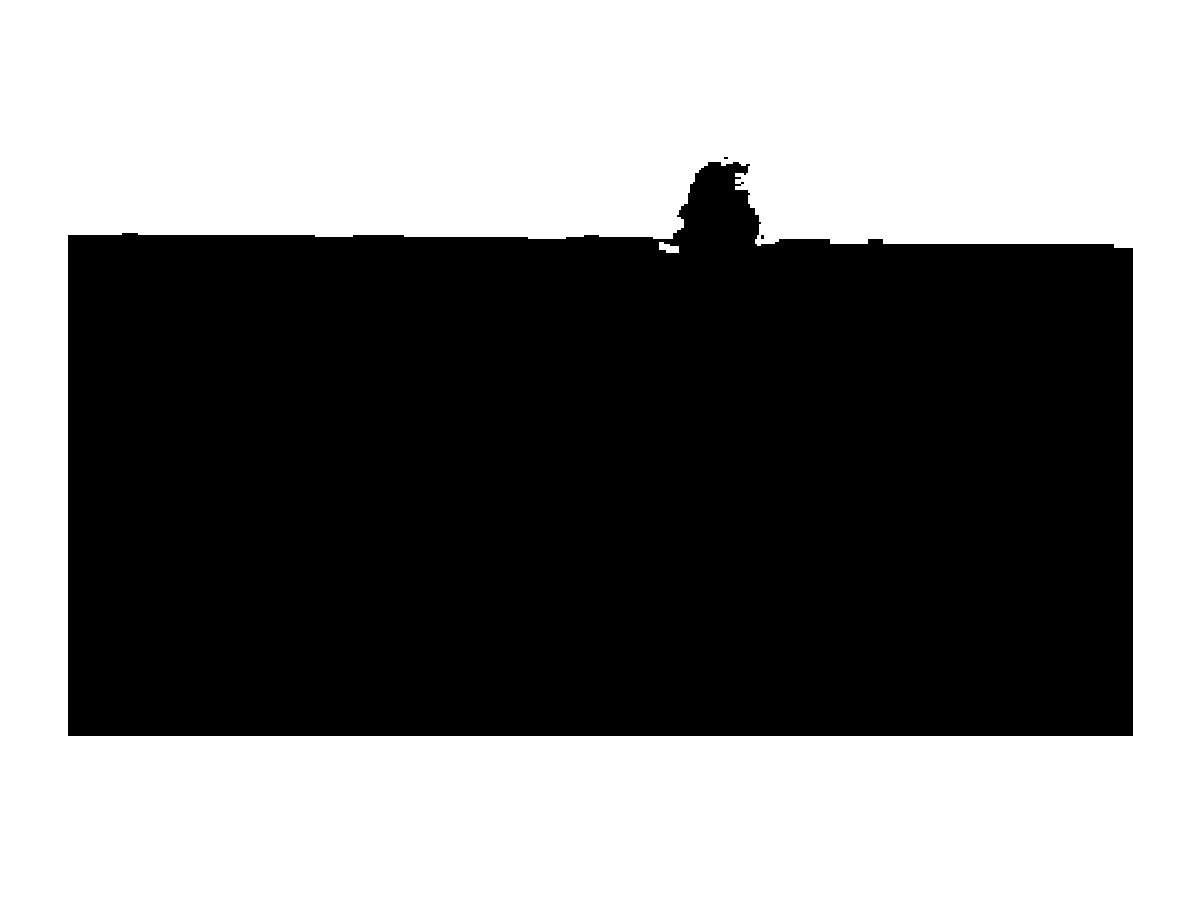
\includegraphics[width=0.16\textwidth]{chap4/depthseg5}}
  \bicaption[fig:segmask]{图\ref{fig:52_L_depthMap:b}产生的图像分割模板}{图\ref{fig:52_L_depthMap:b}产生的图像分割模板}{Fig}{The masks created from\ref{fig:52_L_depthMap:b} }
\end{figure}
\begin{figure}
  \centering
  \subfigure[]{
    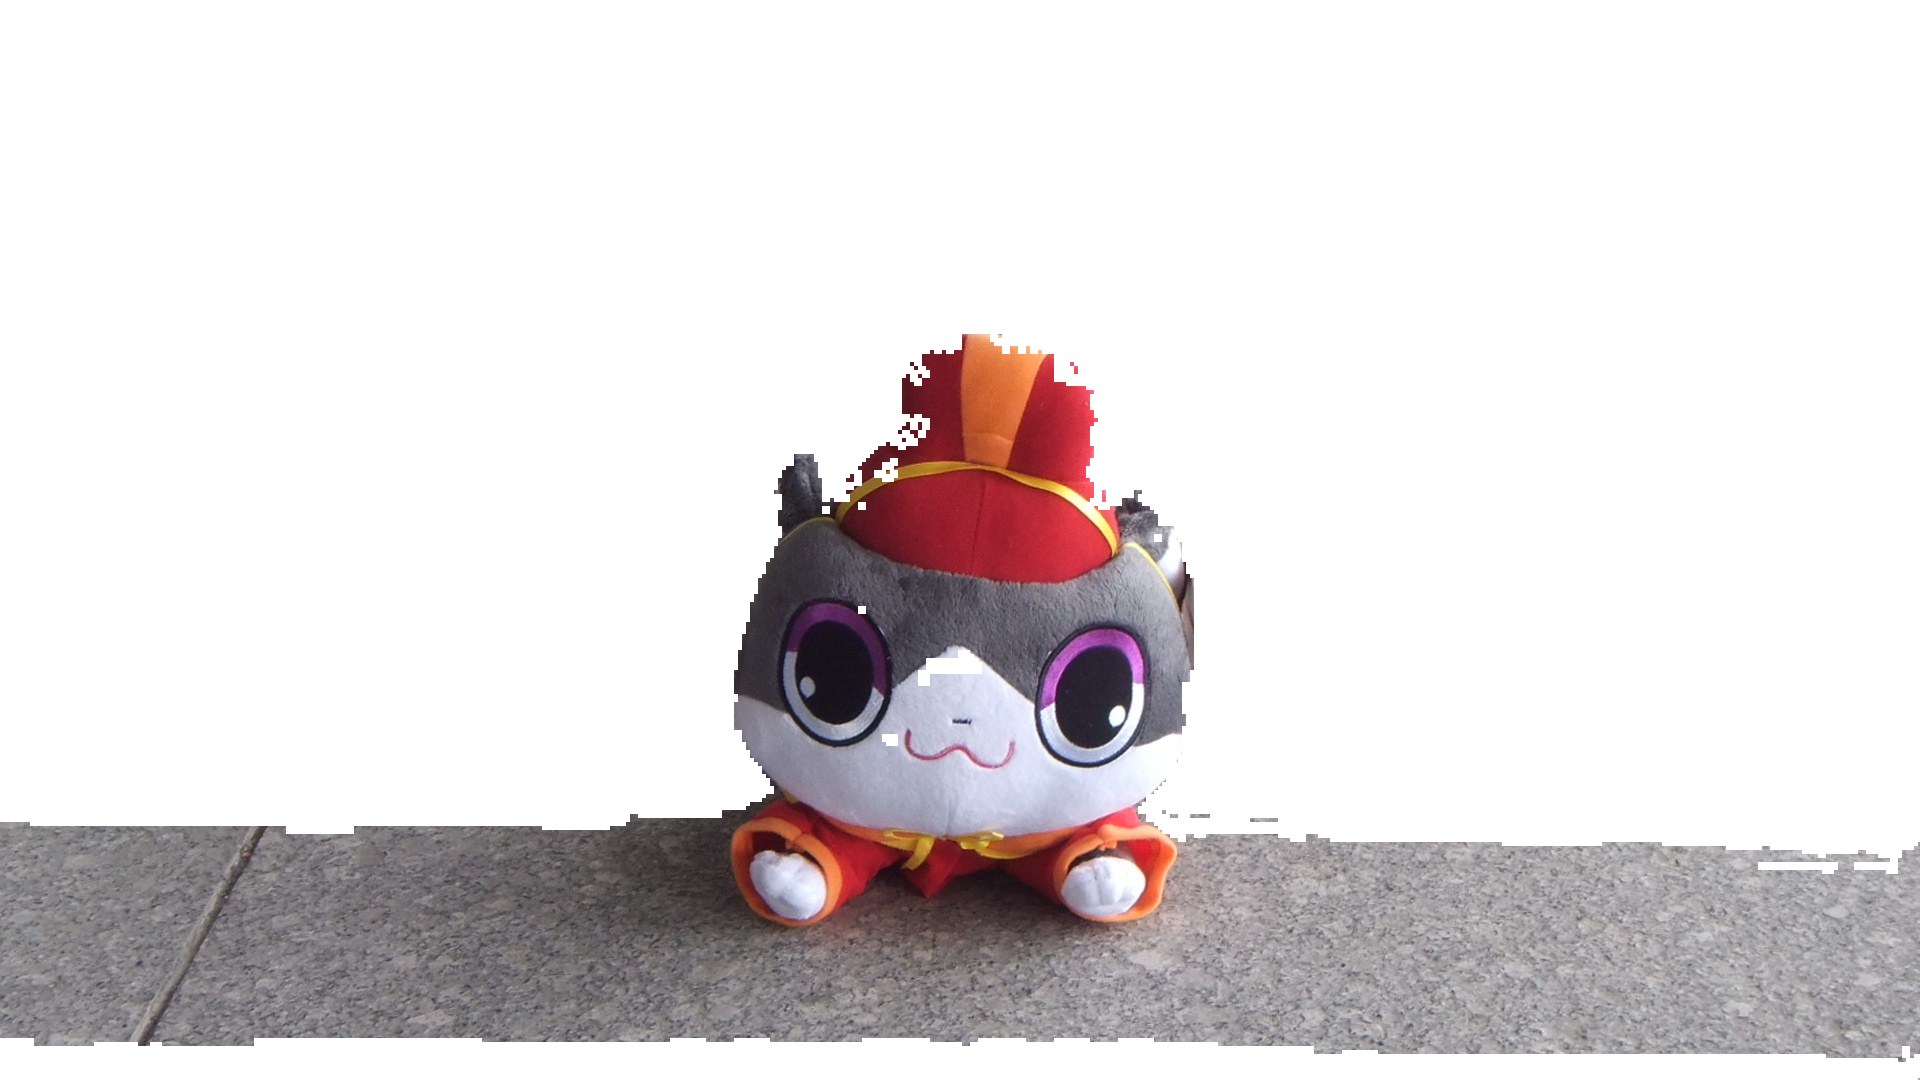
\includegraphics[width=0.16\textwidth]{chap4/testlevel1}}
  \subfigure[]{
    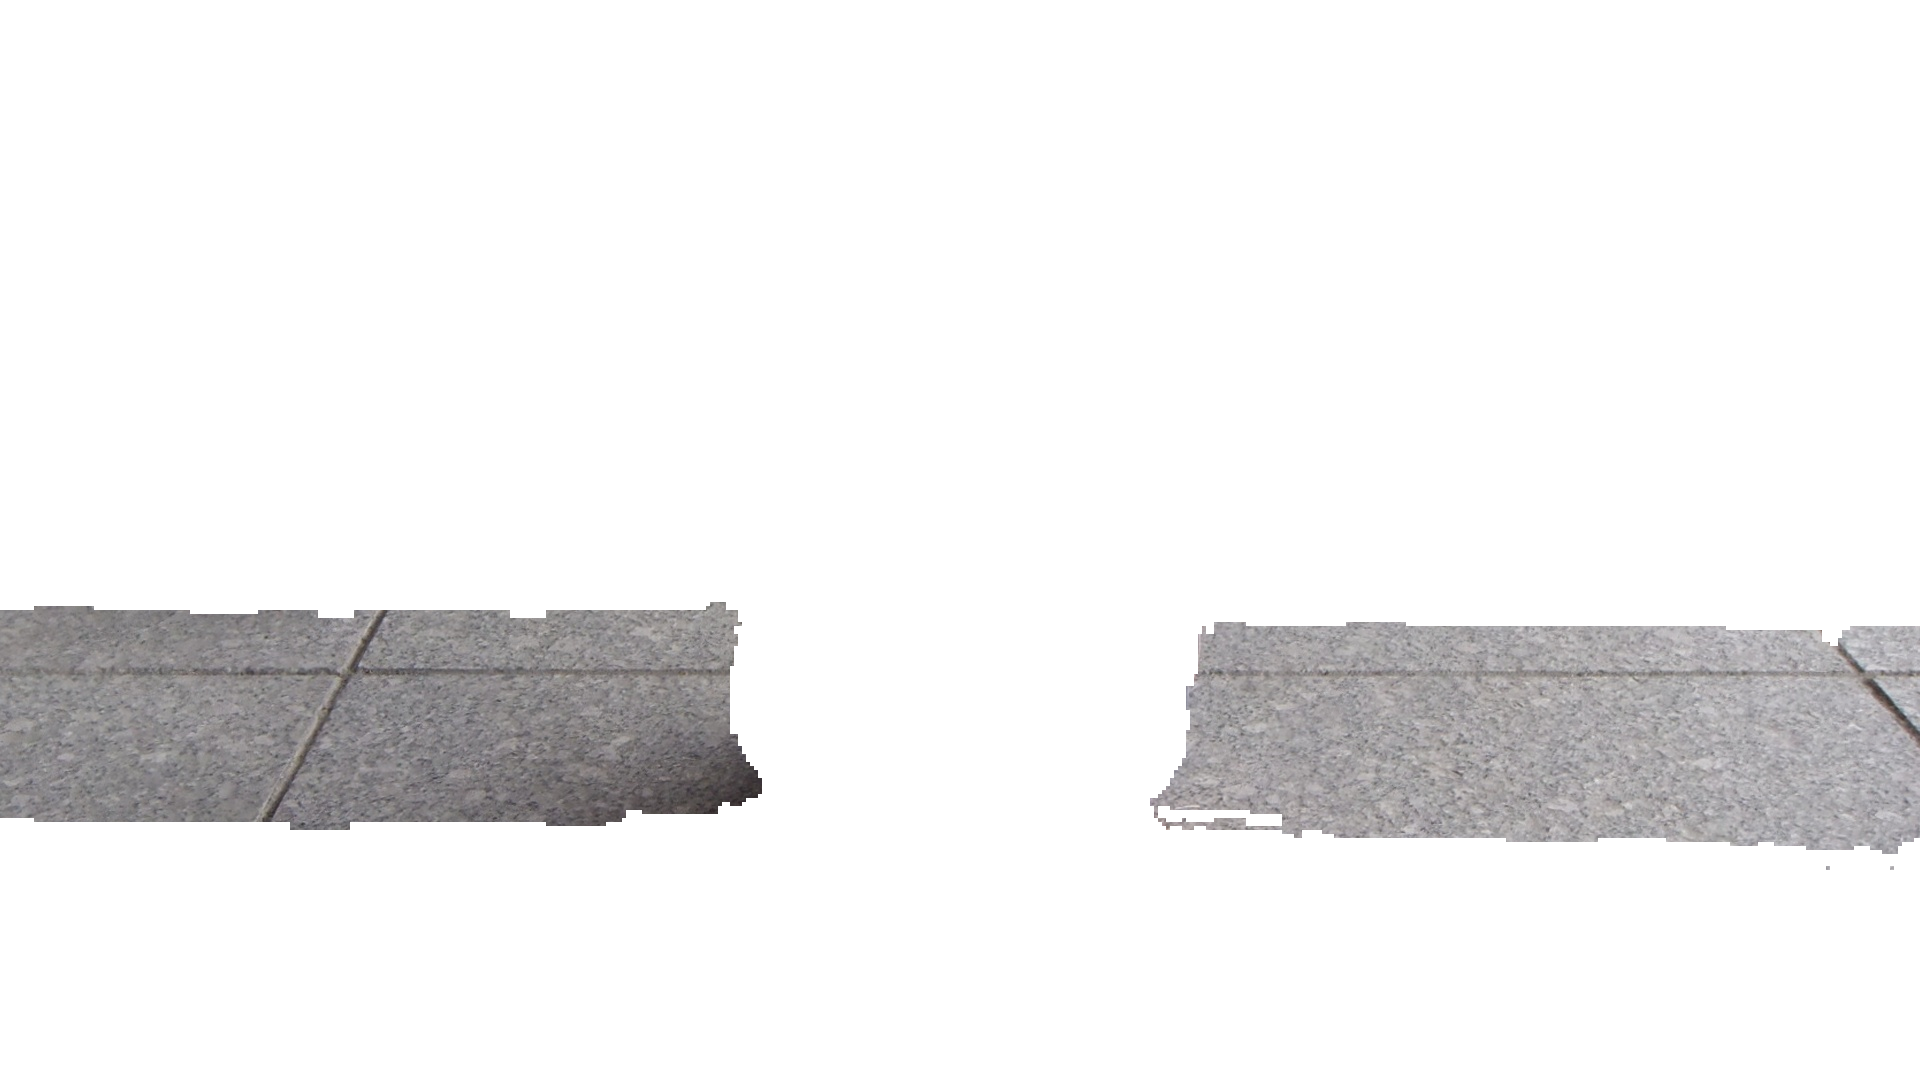
\includegraphics[width=0.16\textwidth]{chap4/testlevel2}}
  \subfigure[]{
    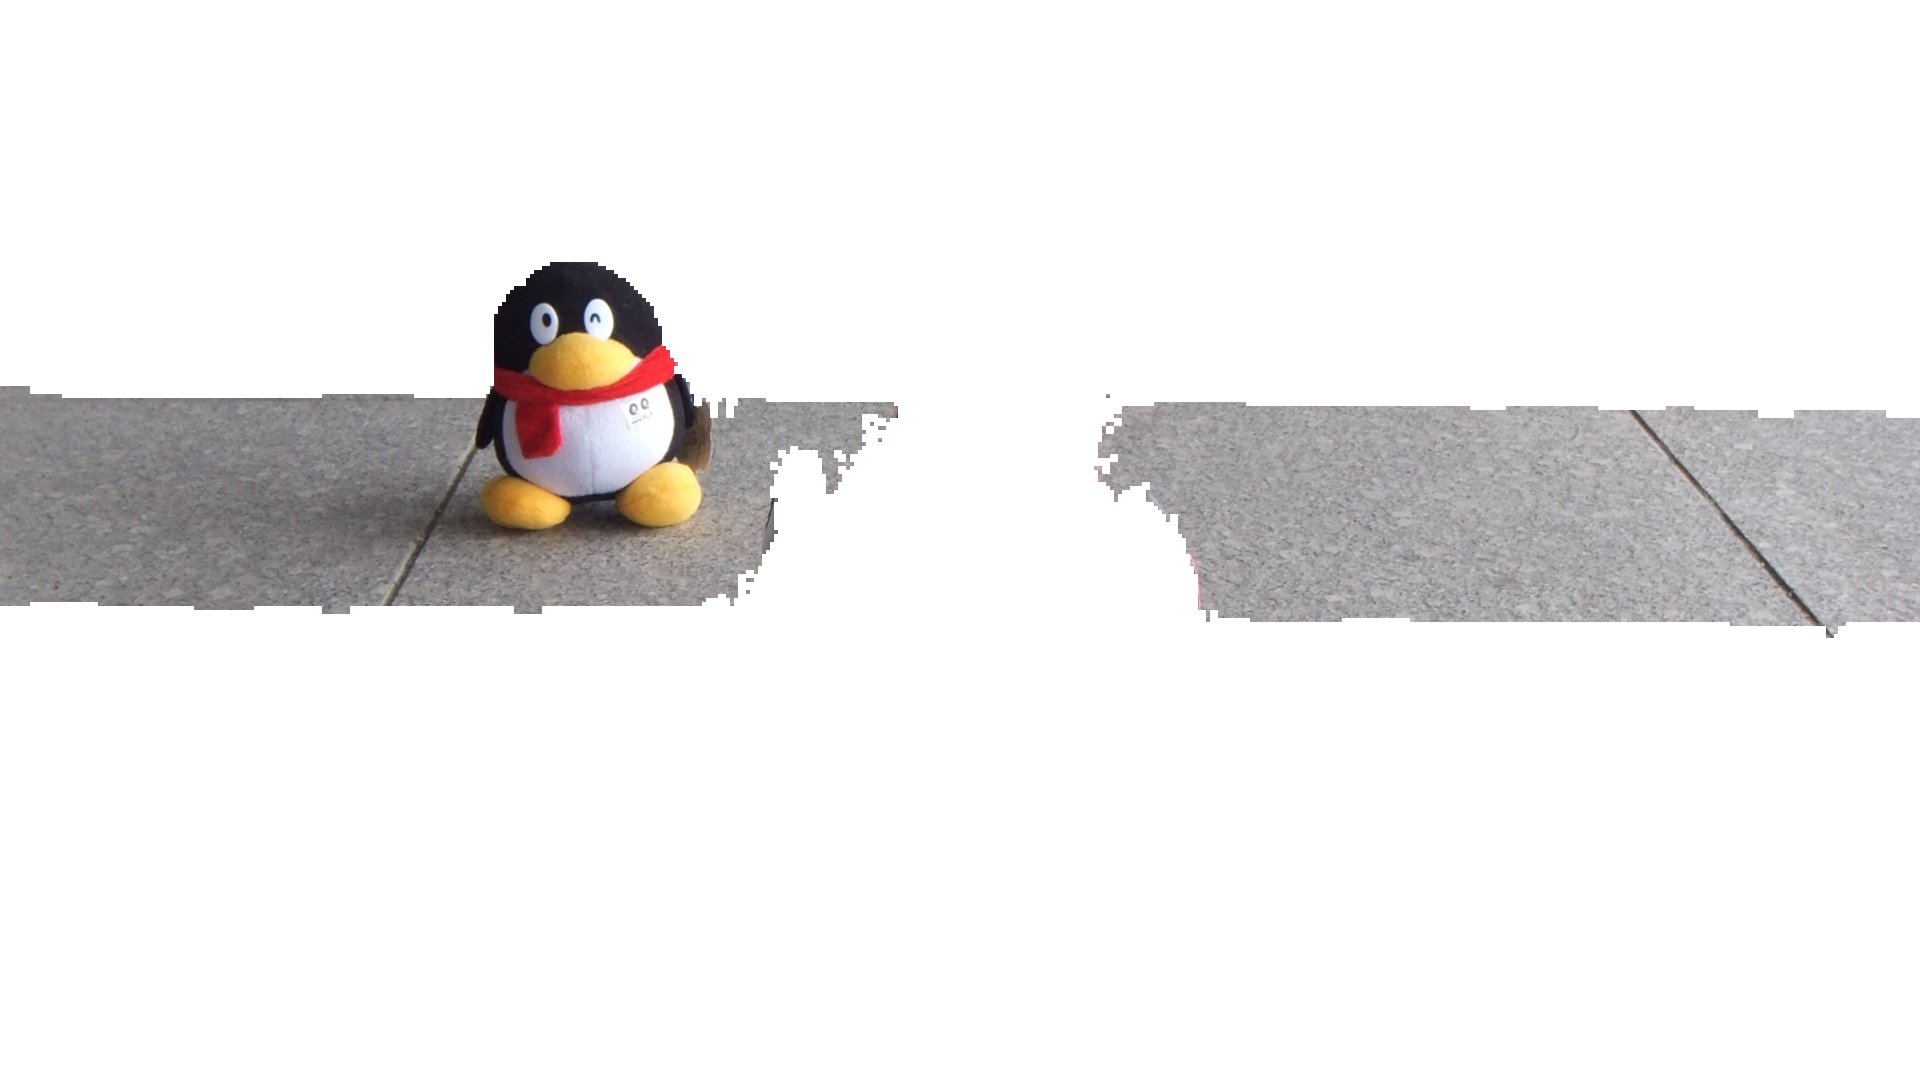
\includegraphics[width=0.16\textwidth]{chap4/testlevel3}}
  \subfigure[]{
    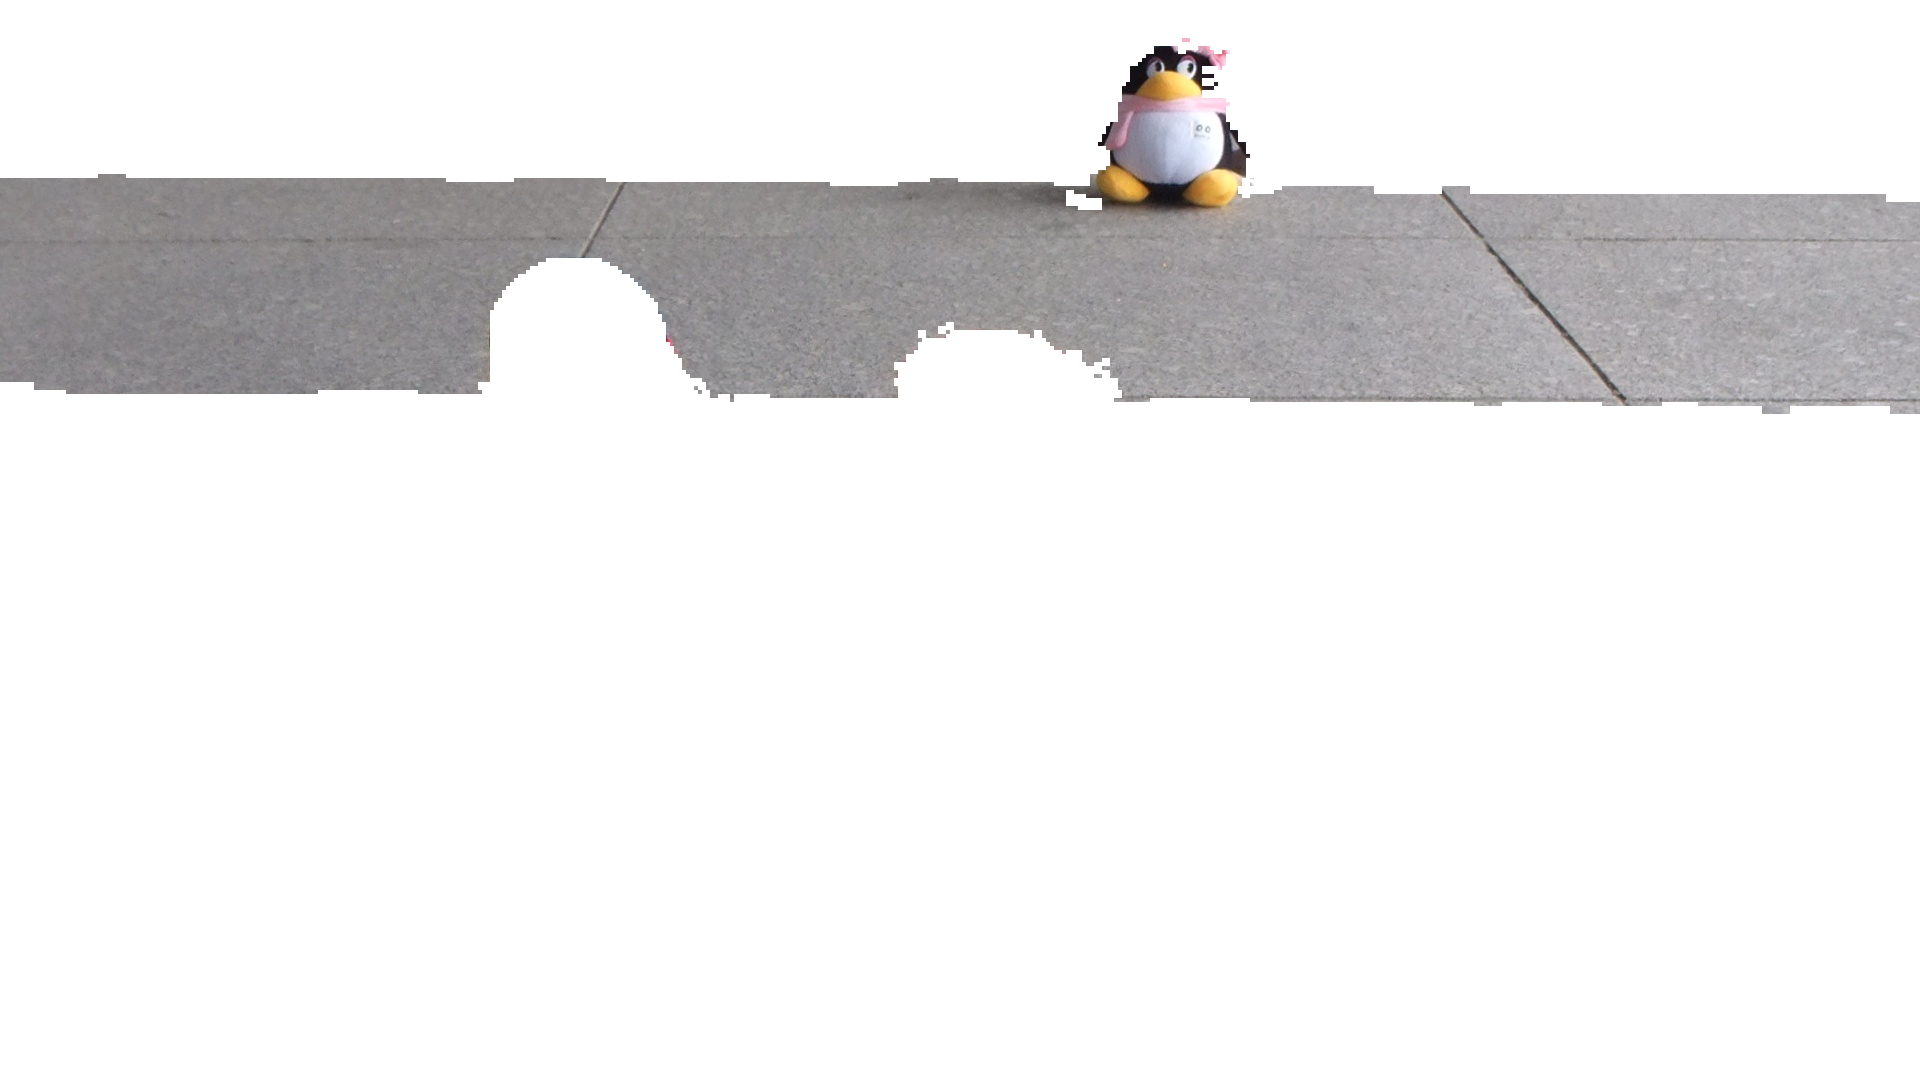
\includegraphics[width=0.16\textwidth]{chap4/testlevel4}}
  \subfigure[]{
    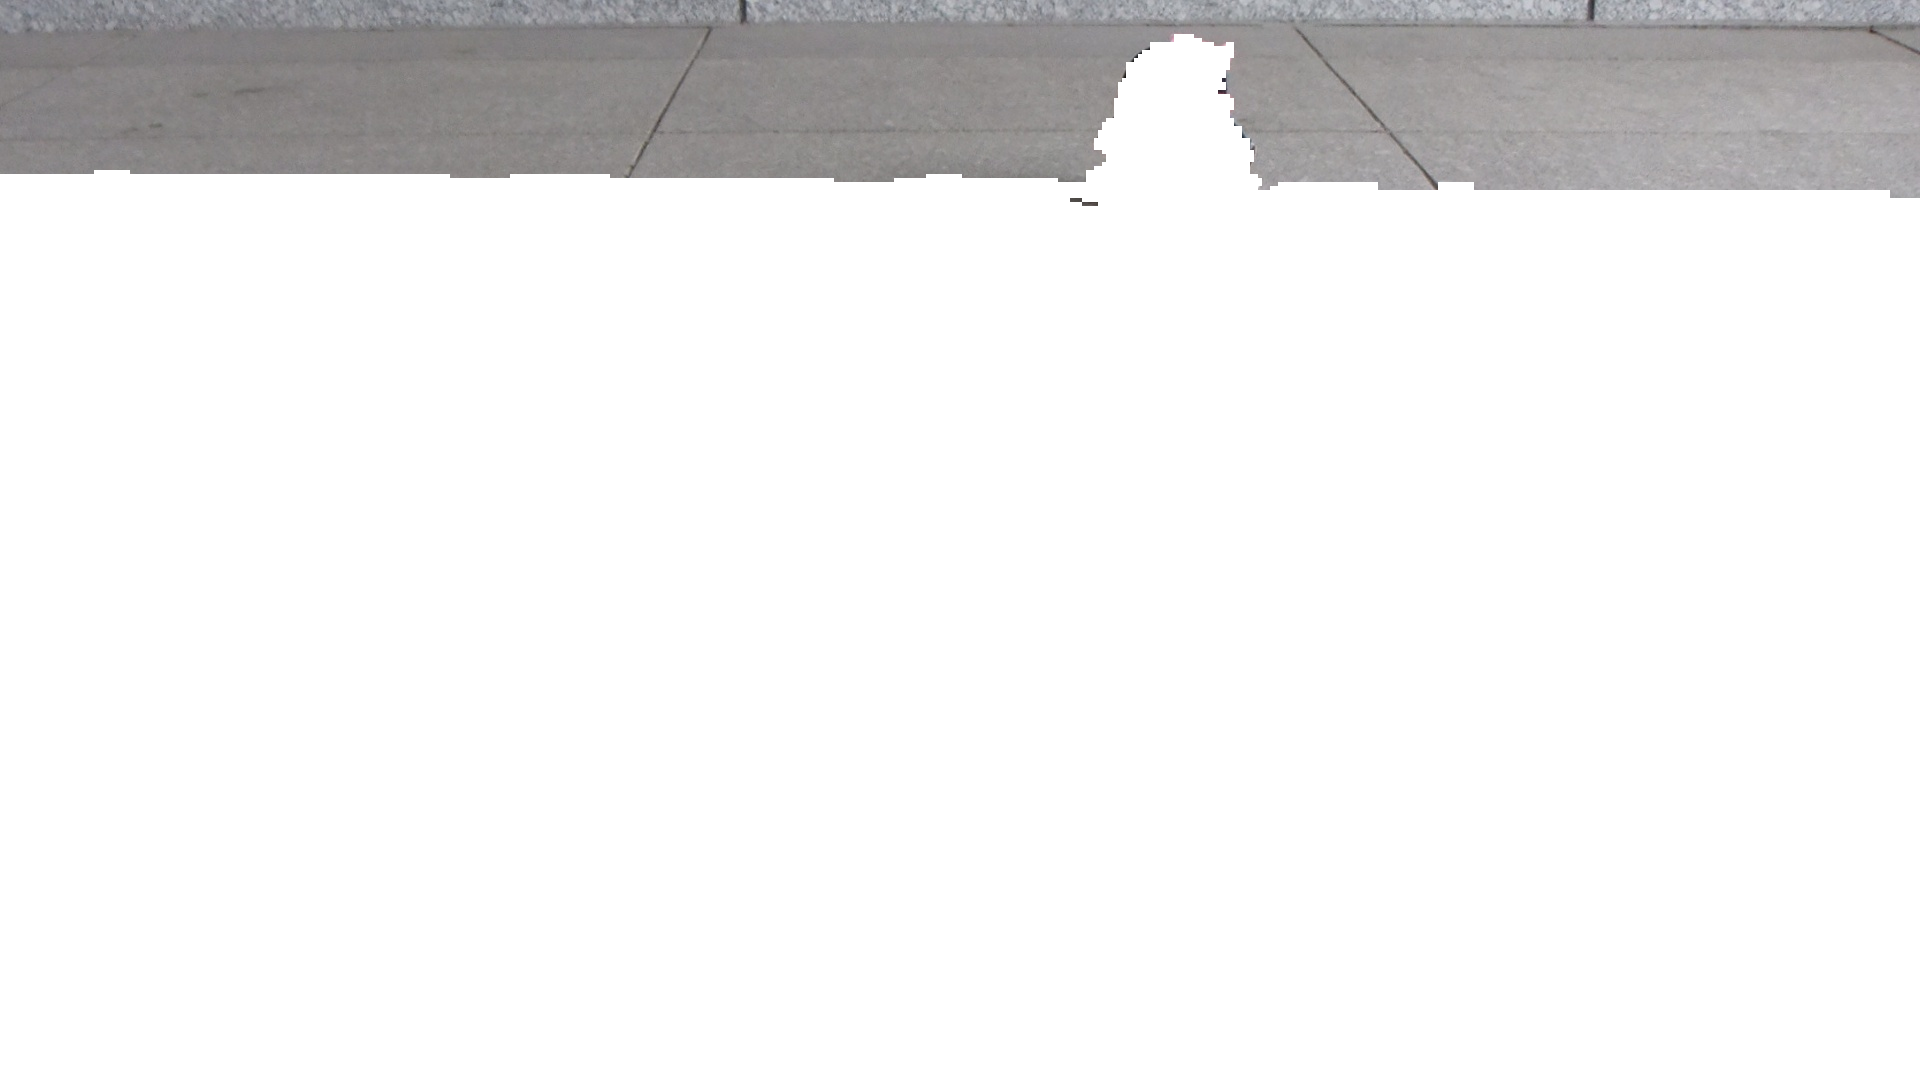
\includegraphics[width=0.16\textwidth]{chap4/testlevel5}}
  \bicaption[fig:segresult]{图\ref{fig:52L:a}分割的结果}{图\ref{fig:52L:a}分割的结果}{Fig}{The result of \ref{fig:52L:a} segmented}
\end{figure}
%%%%%%
\\[0.2cm]
\noindent{\textbf{\emph{e.图像分割及其立体表示}}}
\\[0.2cm]
\indent{利用}从\textbf{\emph{e}}部分创建的图像分割模板${M_{{P_i}}}$来分割原彩色图像  $I$,并把它们显示在相应的深度平面上。

\uppercase\expandafter{\romannumeral1}.
第$i^{th}$ 个与深度平面 ${{{P_i}}}$ 对应的分割的图片${S_{{P_i}}}$可以通过下式来决定:
\begin{equation}
{S_{{P_i}}}(x,y) = I(x,y)*{M_{{P_i}}}(x,y).
\end{equation}
图\ref{fig:52L:a}被分割的结果如图\ref{fig:segresult}所示。


\uppercase\expandafter{\romannumeral2}.
创建三维直角坐标系来显示分割好的图片。用坐标系的$X, Y$分别表示图像的宽和高,用 $Z$轴表示图像的深度,深度平面 $z = 0$指的是3D显示屏幕。为了更直观地观察图像各部分的深度,这里将视差角转化为距离,单位为cm。深度平面${P_i}$相对于屏幕的距离 $z_i$ 可以如下计算:
\begin{equation}
{z_i} = \frac{e}{{2tg\frac{{\alpha  - {\theta_{{P_i}}}}}{2}}} - d.
\end{equation}

\uppercase\expandafter{\romannumeral3}.
将分割后的图片${S_{{P_i}}}$显示在相应地深度平面上,就形成了立体图像的分层表示,为了防止前面的平面遮挡后面的部门,我们对分割图片${S_{{P_i}}}(x,y) = 0$ 的区域进行了透明化处理,使效果更加明显。
最终图\ref{fig:52L:a}的立体分层表示结果如图\ref{fig:finalresult}所示。
\begin{figure}[t]
  \centering
  \subfigure[最终结果的正视图]{
    \label{fig:finalresult:a} %% label for first subfigure
    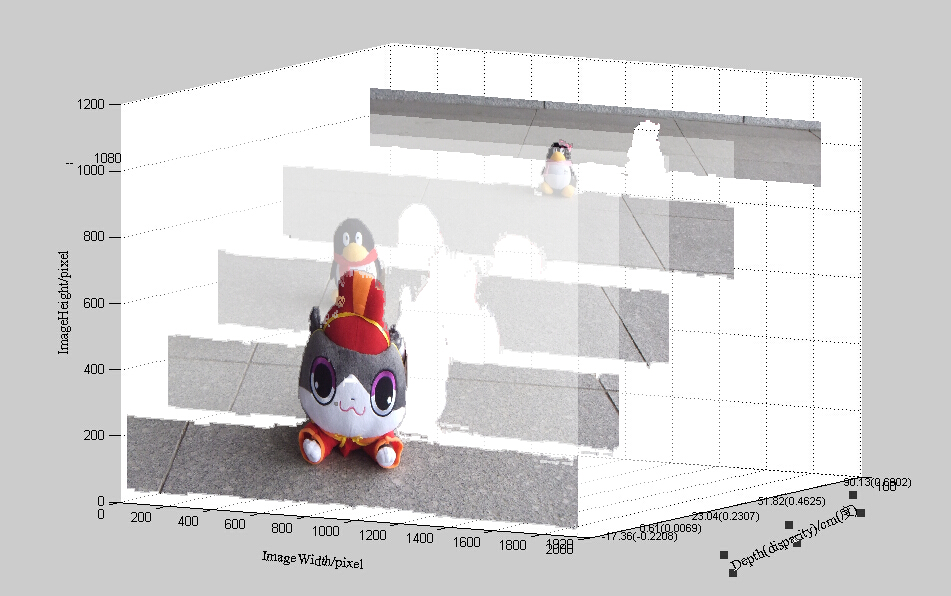
\includegraphics[width=0.4\textwidth]{chap4/finalresult1}}
  \hspace{1in}
  \subfigure[最终结果的侧视图]{
    \label{fig:finalresult1:b} %% label for second subfigure
    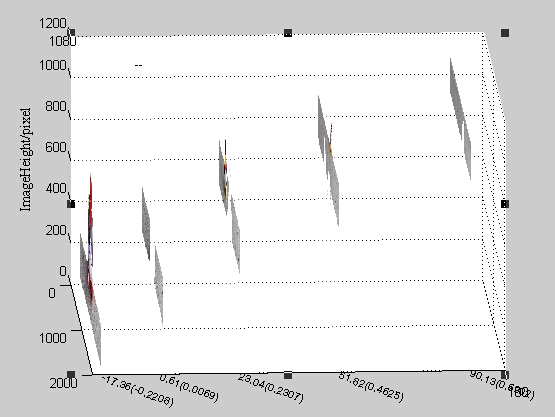
\includegraphics[width=0.4\textwidth]{chap4/finalresult2}}
  \bicaption[fig:finalresult]{图\ref{fig:52L:a}立体分层表示}{图\ref{fig:52L:a}立体分层表示}{Fig}{The multi-layered representation  of \ref{fig:52L:a} segmented}
\end{figure}

\subsubsection{基于立体图像分层的3D注视密度图}
\label{sec:create3Dfixationdensitymap}
现在采用与图像分割类似的方法来创建立体图像的眼动数据注视密度图。
%%%%%%
\\[0.2cm]
\noindent{\textbf{\emph{a.基于视差角的眼动数据分层}}}
\\[0.2cm]
\indent{眼}动数据在使用前要先校正与滤波,具体的方法已经在\ref{sec:calibraiton}  和 \ref{sec:filter}   部分进行了叙述,这里不赘述。

处理后的眼动数据,通过\ref{sec:caldisparity}给出的眼动数据的视差的计算方法获取每个采样点$G_i$的视差角$\theta_i$。然后根据视差角对注视点进行分层。注视点所在层需满足方程\ref{eq:depthplanedisparityrange},这样根据视差角的深度信息,将眼动数据分配在了各自对应的深度平面上。
%%%%%%
\\[0.2cm]
\noindent{\textbf{\emph{b.分层创建2D注视密度图}}}
\\[0.2cm]
\indent{现}在已经获取了对应于各深度平面的图像,也有对应于各个平面的眼动数据,此时,分层创建该深度层次的注视密度图。这个过程采用的是传统的2D注视密度图的方法,即首先创建一个与图像同样大小的矩阵$A$,并初始化为零矩阵,然后对眼动数据序列进行遍历,当视点$G_i$出现在图像的$(x,y)$坐标处时,则$A(x,y)$处加1。这样就可以得到离散的注视点分布图,对该图进行高斯模糊化,并以不同的颜色显示,便可以得到相关的注视密度图。具体的算法如下。
\begin{algorithm}
\caption{ 为深度平面$P_i$创建注视密度图的算法.}
\label{alg:createfdm}
\begin{algorithmic}[1]
\STATE initialize a new array A the same size as stimulu image;
\FOR{each i in[1:length($G_{{P_i}}$)]}
\STATE A(${G_{j}}(x)$,${G_{j}}(y)$)++;Where ${G_{j}}(x)$ and ${G_{j}}(y)$ refer to  horizon and vertical coordinate of gaze point ${G_{j}}$ respectively.
\ENDFOR
\STATE Conv(A,H), where H is a Guassian Kernel;
\label{code:guassian}
\end{algorithmic}
\end{algorithm}
\begin{figure}[t]
  \centering
  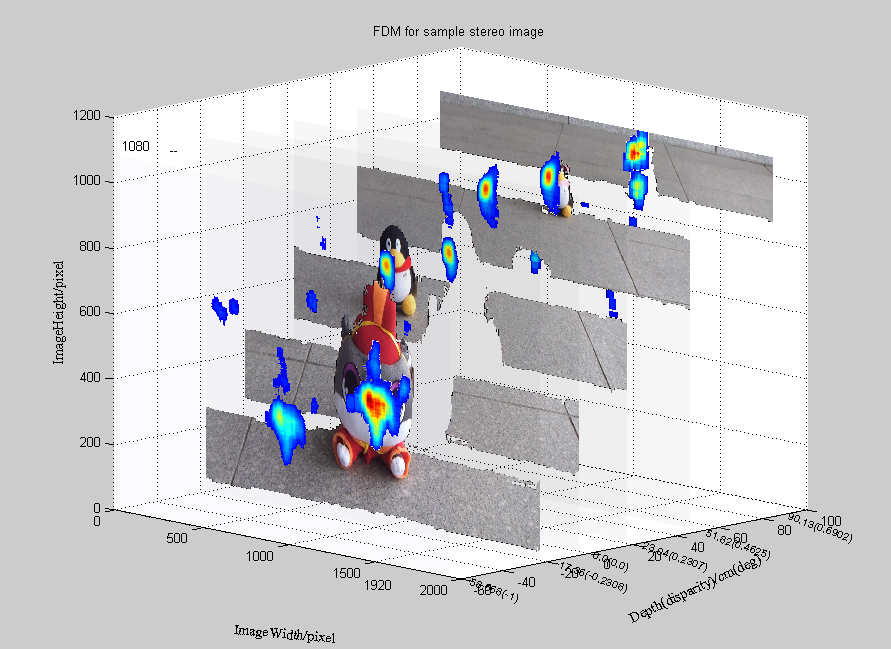
\includegraphics[width=0.5\textwidth]{chap4/fdmresult}
  \bicaption[fig:fdmresult]{图\ref{fig:52L:a}的立体注视密度图}{图\ref{fig:52L:a}的立体注视密度图}{Fig}{The final results of our approach for image\ref{fig:52L:a}}
\end{figure}
%%%%%%
\\[0.2cm]
\noindent{\textbf{\emph{c.创建立体注视密度图}}}
\\[0.2cm]
\indent{和}\ref{sec:stereoscopicimagerepresentation}中\textbf{\emph{e}}的方法一样,将对应于各个深度平面的2D密度注视图联合起来便可以得到立体的注视密度图,图\ref{fig:fdmresult}是正对示例图片\ref{fig:52L:a}创建的注视密度图。
%%%%%%
\\[0.2cm]
\noindent{\textbf{\emph{d.创建立体注视密度图方法小结}}}
\\[0.2cm]
\indent{前}面给出了创建注视密度图的方法,这里小结一下。先来回顾一下目前已有的工具,如表\ref{tools}。
\begin{table}[]
\centering
\caption{目前已有的素材和技术}
\label{tools}
\begin{tabular}{|c|c|c|}
\hline
目前已有的基础  & 所在章节                                & 创建FDM中的功能                                                                   \\ \hline
3D校正实验   & \ref{sec:3dcalibrationexperiment} & 数据校正基础                                                                      \\ \hline
立体图像眼动数据 & \ref{sec:3dcalibrationexperiment} & FDM的基本素材                                                                    \\ \hline
眼动数据校正   & \ref{sec:calibraiton}             & \begin{tabular}[c]{@{}c@{}}利用3D校正实验的数据获取个人校正\\ 系统并纠正该被试的所有眼动数据\end{tabular} \\ \hline
眼动数据滤波   & \ref{sec:filter}                  & 除去眼动数据中的噪声,并分离出注视与扫视过程                                                      \\ \hline
立体图像分层表示 & \ref{sec:stereoscopicimagerepresentation}            & FDM骨架                                                                       \\ \hline
\end{tabular}
\end{table}
现在,我们来创建任意一副测试图片的平均注视密度图。

第一,通过实验3D校正实验(\ref{sec:3dcalibrationexperiment})收集的所有被试的眼动数据,针对每个人利用眼动数据3D校正方法 (\ref{sec:calibraiton} )获取该用户的校正偏差系统系数,对该用户的所有立体图像下的眼动数据(\ref{sec:3dcalibrationexperiment})进行校正,得到新的校正过的眼动数据集$\Phi'$;

第二,对第一步处理后的眼动数据集,采用眼动数据滤波( \ref{sec:filter})算法进行除噪和眼动过程分离得到注视过程和扫视过程,此时的数据构成滤波过的眼动数据集$\Phi''$;

第三,选择要创建注视密度图的立体图像$I$(左图或右图),并利用\ref{sec:stereoscopicimagerepresentation}  中的方法创建该图像的分层表示。

第四,从$\Phi''$中选出与该图片对应的所有用户的眼动数据,求取眼动数据的视差角,并依据第三步中的分层结点对眼动数据进行分层。

第五,在各深度平面上创建2D注视密度图,然后将各层密度图结合形成立体盒子,这样就可以得到立体的注视密度图。

\section{眼动实验结果分析}
\label{sec:resultshow}
本章的\ref{sec:eyetrackdataprocess}研究了眼动数据的基本处理技术,在对眼动数据进行了校正和滤波之后,我们提出了一种基于分层表示的立体图像创建3D注视密度图的方法。本节将通过这种方法来对眼动数据结果做一些分析。

图\ref{fig:69s11}和图\ref{fig:82s-11}是我们实验中用到的两幅立体图像的左图,图\ref{fig:69s11}是一个总体深度较大的风景图片,其视差特征是:两侧视差梯度较大,而中间视差总体上变化不大。而图\ref{fig:82s-11}是画面内容比较丰富的集市场景,由于多目标的关系,视差在局部区域变化明显。图\ref{fig:fdmanalysisfor69s11}和图\ref{fig:fdmanalysisfor82s-11}是相应的从不同角度来看的注视密度图。我们据此来分析一下其中的眼动特征。
\begin{figure}
  \centering
  \subfigure[69s11.jpg左图]{
   \label{fig:69s11}
    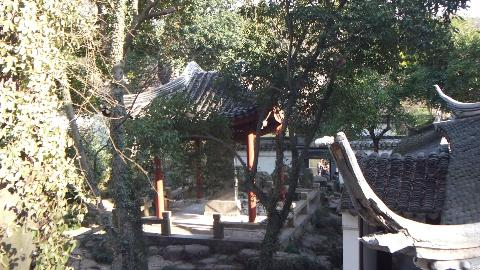
\includegraphics[width=0.4\textwidth]{chap4/69s11}}
  \subfigure[82s-11.jpg左图]{
   \label{fig:82s-11}
    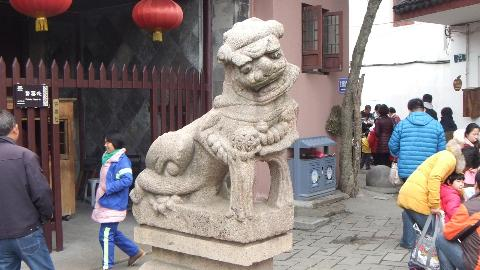
\includegraphics[width=0.4\textwidth]{chap4/82s-22}}
  \bicaption[fig:69s11vs82s-11]{实验原图的示例图像}{实验原图的示例图像}{Fig}{The Original Image }
\end{figure}
\begin{figure}[t]
  \centering
  \subfigure[FDM1 for 69s11.jpg]{
   \label{fig:fdm1for69s11}
    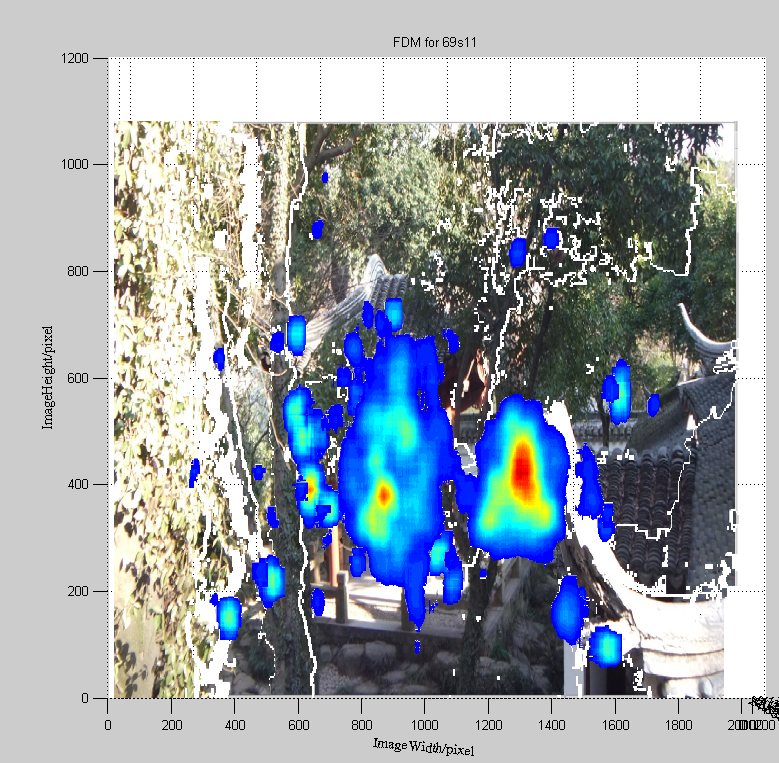
\includegraphics[width=0.28\textwidth]{chap4/fdmfor69s11front}}
  \subfigure[FDM2 for 69s11.jpg]{
   \label{fig:fdm2for69s11}
    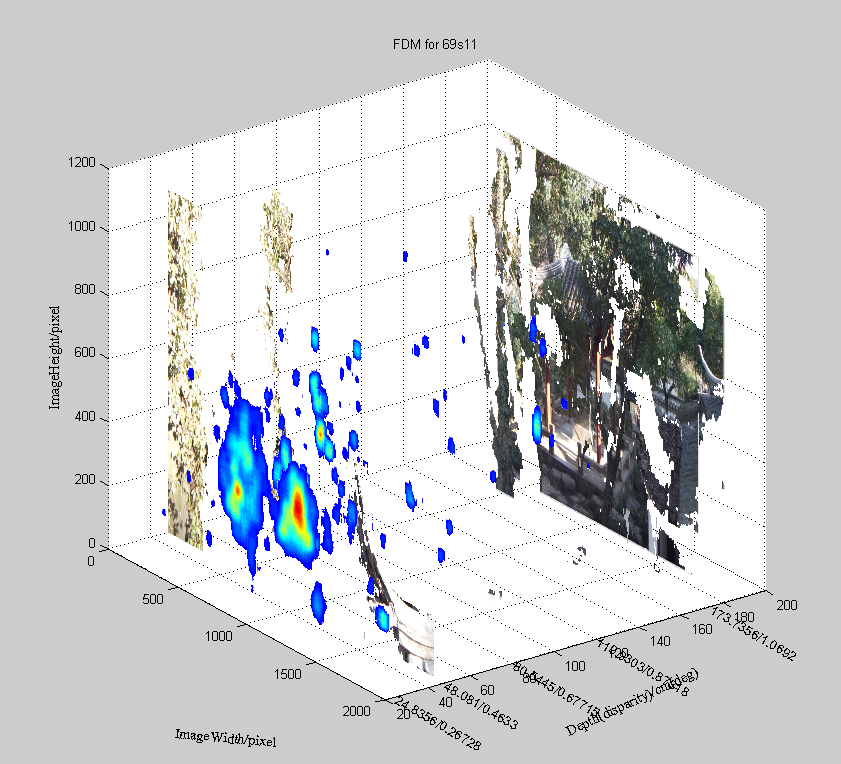
\includegraphics[width=0.3\textwidth]{chap4/fdmfor69s11}}
  \subfigure[FDM3 for 69s11.jpg]{
   \label{fig:fdm3for69s11}
    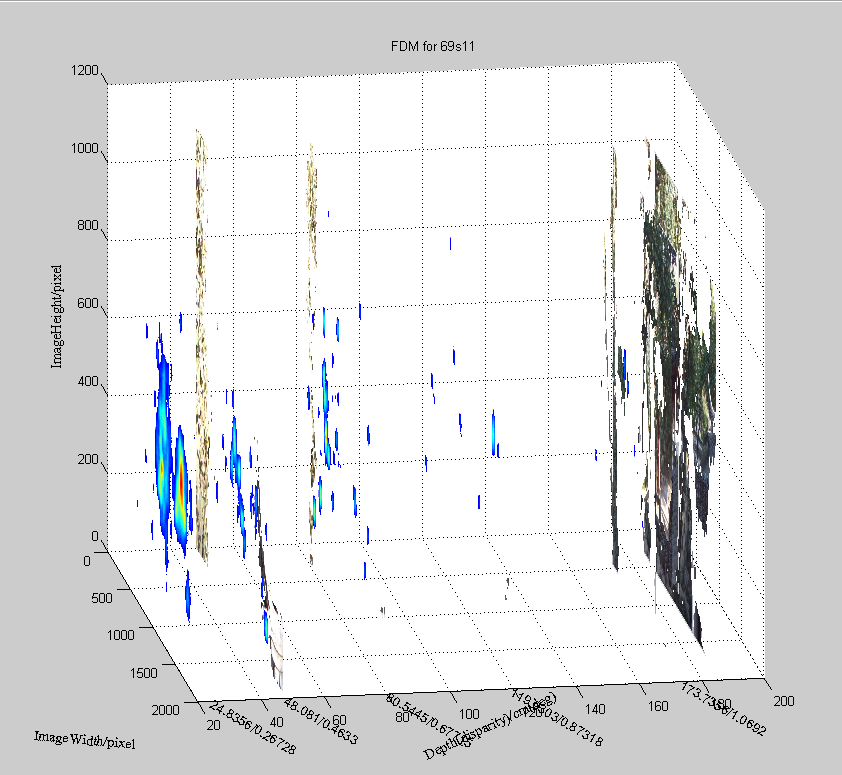
\includegraphics[width=0.3\textwidth]{chap4/fdmfor69s11neighbor}}
  \bicaption[fig:fdmanalysisfor69s11]{\ref{fig:69s11}的不同角度的FDM图}{\ref{fig:69s11}的不同角度的FDM图}{Fig}{The FDMs for \ref{fig:69s11} }
\end{figure}
\begin{figure}[ht]
  \centering
  \subfigure[FDM1 for 82s-11.jpg]{
   \label{fig:fdm1for82s-11}
    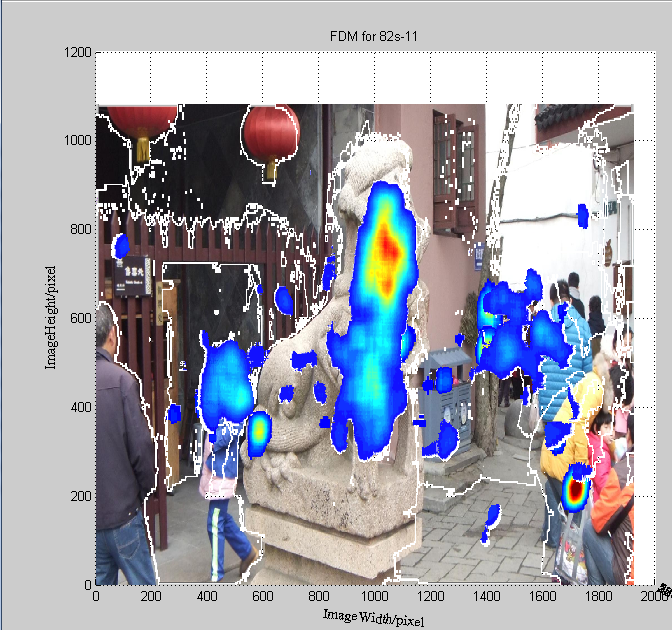
\includegraphics[width=0.3\textwidth]{chap4/fdmfor82s-11front}}
  \subfigure[FDM2 for 82s-11.jpg]{
   \label{fig:fdm2for82s-11}
    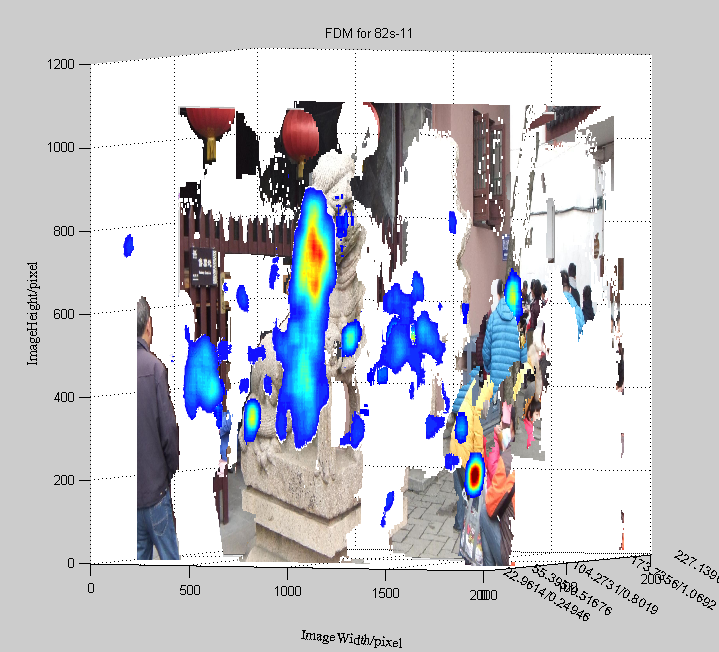
\includegraphics[width=0.3\textwidth]{chap4/fdmfor82s-11}}
  \subfigure[FDM3 for 82s-11.jpg]{
   \label{fig:fdm3for82s-11}
    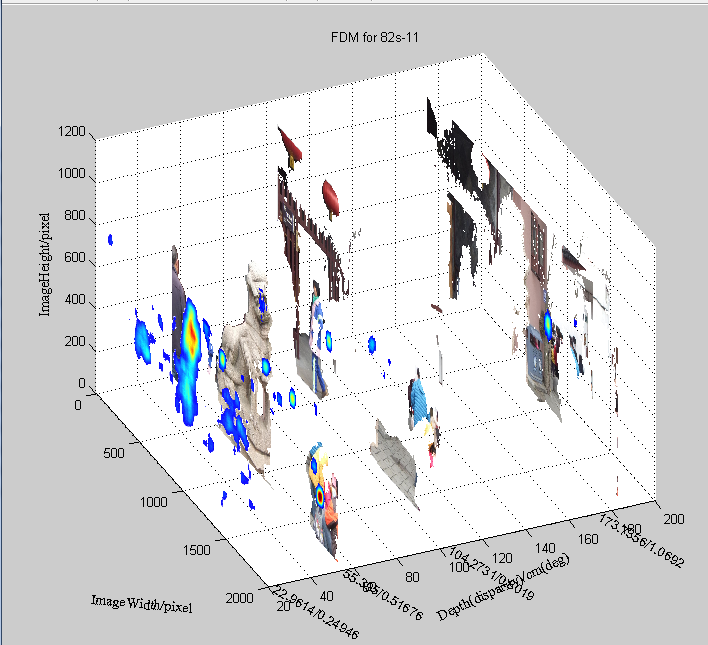
\includegraphics[width=0.3\textwidth]{chap4/fdmfor82s-11neighbor}}
  \bicaption[fig:fdmanalysisfor82s-11]{\ref{fig:82s-11}的不同角度的FDM图}{\ref{fig:82s-11}的不同角度的FDM图}{Fig}{The FDMs for \ref{fig:82s-11} of different views.}
\end{figure}

图\ref{fig:fdm1for69s11}和图\ref{fig:fdm1for82s-11}是相应的注视密度图的正视图,我们发现,当所有的深度平面在深度方向合并后,此时的深度平面只有一个,原立体的密度注视图退化成了2D注视密度图。因此,本文的方法是一种更高维度的方法,2D注视密度图可以看成是3D注视密度图的一种特殊情况。2D注视密度图结果显示,人眼在图 \ref{fig:69s11}的注视区域集中在“凉亭”上,从图像内容来看,“凉亭”位于图像中央,人眼注视图像中央是合理的。但是,和旁边的“树木”相比,“凉亭”所处区域的视差变化相对较小。Liu\parencite{liu2010scene}的工作已经证明了人眼比较喜欢注视亮度对比度和梯度比较大的区域,但在视差方面却是相反的,即人眼喜欢注视视差对比度和梯度较小的区域。我们的观察结果也印证了这一点。同样的结果在图\ref{fig:82s-11}也观察到了,人眼在“石狮”身上的注视程度远高于后面的“人群”等,“石狮”的视差变化较小是造成这种情况的原因之一。

图\ref{fig:fdm2for69s11}和图\ref{fig:fdm2for82s-11}是相应的注视密度图侧转${45^ \circ }$后的结果。此时我们发现,大部分眼动数据集中在视差角比较小的范围,造成这种情况的原因有两种可能:一是眼动数据测量不准确,目前的眼动仪的精度确实没有那么高,所以存在测量偏差在所难免。但是生理学的发展给了另一种解释这种情况的角度。生理学家将“视差”这个概念细分为“绝对视差”与“相对视差”两种类型。“绝对视差”的意思是可以定量地分辨出两个不同深度的物体的深度差,“相对视差”的意思是人眼只是可以分辨出两个物体的远近。Westheime\parencite{westheimer1979cooperative}证明了人眼的相对视差视敏度是绝对视差视敏度的5倍,这与通常的认知和体会是相符的。我们可以轻易获取两个物体的远近,而绝对深度差则往往没有那么准确。所以,人眼在观看的时候只要感知到视野中物体的远近即可,然后眼睛就会停留在相对舒适的区域,而无需调整眼睛去适应绝对视差值。这正是我们观察到的结果。

我们再来看图\ref{fig:fdm3for69s11}和图\ref{fig:fdm3for82s-11},它们是相应的注视密度图侧转${80^ \circ }$的结果。我们发现达到较大深度的注视点很少。特别是\ref{fig:fdm3for69s11},其最后的背景超出了立体舒适度范围$( - 1^\circ , + 1^\circ )$,此时,几乎没有眼动数据的视差达到这个范围。除了人眼感知相对视差的原因之外,Filip- pini 和 Banks\parencite{filippini2009limits}给出了一个更加出名的解释:当一个区域的视差变化很大的时候,眼睛是不会去感知这种视差变化的。这正是立体注视密度图反映出来的情况。同时这也解释了当我们看理论上已经超出汇聚条件的图片时,眼睛依然可以聚焦。这是眼睛进行了视差选择,即忽略了大视差的区域,只在大脑中形成一个相对视差的印象,而眼睛依然停留在较舒适的范围。这个过程类似于图像传输过程中压缩的原理。

以上我们结合注视密度图对眼动数据的深度分布进行了解释。我们发现,眼动数据的视差大多集中在绝对视差角较小的区域。而这既是图像本身信息分布决定的结果,也是眼睛自身生理特征的结果。眼动数据的视差角与图像的视差既有联系又有区别,联系是眼睛要去感知相对视差,所以,眼动数据中一定会有大视差角变化的过程(当然前提是图像本身是大视差的),区别是眼睛并不会随着视差的增加而去迎合这种增大或者长时间去适应这种增大。无论如何,眼动数据的视差角在立体视觉中扮演了很重要的角色。这为我们在第\ref{chap:model}章提取眼动特征来评价立体图像质量奠定了基础。

\section{总结}
\label{sec:conclusionchapter4}
本章主要对实验数据进行了处理,主要是对主观评分与眼动数据进行了处理。

首先利用ITU-R BT.500-11的标准方法对主观评分进行了异常值检测。第一,获取每幅图像的峰度,根据峰度判断每幅图像主观评分的分布;第二,基于分布类型设定了判定主观评分是否有效的临界点,利用每幅图像的临界点,获取每个被试在测试过程中评分的偏差次数。第三,检验了每个被试局部偏差——偏大(小)的程度,没有发现异常测试。最后,利用绝对偏差系数和相对偏差系数来度量了每个用户的偏差程度。最终发现,没有数据符合异常拒绝规则。在此基础上,获取了每幅图像的MOS值。

眼动数据的处理是本章的重点。
首先,直接剔除测量过程可能引入噪声的过程的数据。在3D校正实验中,每个“目标”的播放的开始阶段,由于准确追踪目标需要时间,所以可能引入噪声。在立体图像眼动实验中,图像播放的开始受上幅图像的影响可能引入噪声,在图像播放结束时,由于观看时间较长引起的视觉疲劳,被试者的注意力下降,也可能引入噪声,因此,剔除图像播放开始与结束各1s 的数据。

其次,利用3D校正实验的数据获取每个人测量过程中的深度系统偏差,并用此对立体图像眼动实验数据进行了校正。眼动数据进行3D校正的原因是目前的眼动仪是针对2D播放场景设计的,因此,眼动仪一般只有2D校正过程。3D校正的思想是:预先在不同深度平面的不同位置设置“目标”,根据立体成像原理,可以预先获得这些目标对应的深度,实验过程中测量的数据也可以计算当前眼动数据反映的深度,对二者利用拉格朗日最小均方差就可以获取系统偏差,从而使用系统偏差校正立体图像的眼动数据。

再次,对眼动数据进行了滤波。眼动数据的滤波的目的是除噪与眼动过程分离。本章讨论了眼动数据的噪声后发现,眼睛注视点的横纵坐标均符合正态分布,也就是说,眼动数据包含的噪声是高斯噪声。我们利用了\parencite{olsson2007real}中的方法,该方法将眼动过程分离与去噪合二为一,利用了注视点间距固定窗的累积和最大时对应的眼动过程为扫视过程这一特性,将眼动过程分为注视过程与扫视过程。注视过程用注视序列的中位点来估计,这相当于利用中值滤波去除了高斯噪声。我们还建议滤波时采用辅眼作为参考眼,这个建议来自于第\ref{chap:model}章的结果分析——依据辅眼滤波的眼动数据特征表现更好。

最后,给出了一种基于立体图像分层表示的3D注视密度图的创建方法。此方法的提出是为了表示眼动数据的深度信息。为了创建这种密度图,首先提出了一种基于视差分割的立体图像的立体分层表示方法。该方法在提取立体图像视差图后,估计出了用于表示该立体图像的深度区间,在考虑舒适性等因素的情况下,依据人眼立体视敏度将深度空间分为若干个等级,并据此将视差图也分割成相应的等级,从而创建了立体图像分割模板,利用模板将图像分割成对应于相应深度平面的若干份。最后将图像在空间直角坐标系中表示出来。这样,图像内容的深度就可以近似的用相应深度平面的深度信息估计。在获取图像的立体表示之后,利用同样的方法,根据眼动数据计算的视差角将眼动注视点分配在了相应的深度平面上,并在各深度平面创建了平面注视密度图,将各个深度平面合成就可以得到眼动数据的3D注视密度图。利用这些密度图,结合已有的生理学的基本原理,对眼动过程进行了相应的分析,结果发现,眼动数据记录的眼动过程与目前生理学的结论是一致的。除此之外,我们在这种图上发现了视差角分布的特点——大部分集中在零视差平面附近,偶尔会出现大视差的特征,这为了在第\ref{chap:model}章提取眼动数据的视差特征奠定了基础。

本章的工作是眼动数据处理与应用的基础,每个环节的处理效果都会影响到最终的应用。在这方面还有许多工作需要补充。